\documentclass{beamer}
\usepackage[utf8]{inputenc}
%\usefonttheme{serif}
\usefonttheme{professionalfonts}
\setbeamertemplate{navigation symbols}{}
\setbeamertemplate{headline}{}
\setbeamertemplate{caption}[numbered]
\setbeamertemplate{footline}[frame number]
\usepackage{hyperref}
\usepackage{subcaption}
\usepackage{cleveref}
\usepackage{amsmath}
\usepackage{appendixnumberbeamer}
\usepackage{amssymb}
\usepackage{tikz}
\usepackage{wrapfig}
\usepackage{tabularx}
\usepackage{siunitx}
\usepackage{xcolor}
\usepackage{siunitx}
\usepackage{nicefrac}
\usepackage{bm}
\usepackage{cprotect}
\usepackage{caption}
\setlength{\parskip}{8pt}
\setlength{\parindent}{0pt}
\captionsetup{font=scriptsize,labelfont=bf}
%\usefonttheme{serif}
\usecolortheme{seahorse}

% Units definitions
\DeclareSIUnit \parsec {pc}
\DeclareSIUnit \magnitudes {mag}
\DeclareSIUnit \gauss {G}

\makeatletter
\let\org@parboxrestore\@parboxrestore
\def\@parboxrestore{%
\edef\restore@parsettings{%
\parindent=\the\parindent\relax
\parskip=\the\parskip\relax
}%
\org@parboxrestore
\restore@parsettings
}
\makeatother

\setbeamertemplate{frametitle continuation}{}


\newcommand\matr[1]{\ensuremath{\boldsymbol{\mathbf{#1}}}}
\newcommand\vect[1]{\ensuremath{\bm{#1}}}
\newcommand\dint{\ensuremath{\int\displaylimits}}


\title{Investigation of the solar atmosphere using machine learning techniques}
\author{Daniel Zahnd}
\date{January 31, 2024}

\begin{document}

\begin{frame}[noframenumbering, plain]
\maketitle
\end{frame}
\setcounter{framenumber}{0}

\setlength{\parskip}{2pt}
\begin{frame}{Content}
\tableofcontents
\end{frame}
\setlength{\parskip}{8pt}
\section{Introduction}
\begin{frame}[allowframebreaks]{Introduction}
Space weather relies on identification of precursors to solar eruptions.

Inversions (conversion of observations into physical parameters) are needed to identify those precursors.

Most inversion models need to be inverted numerically; conventional methods are computationally costly.

This thesis explores the application of a machine learning technique called ``normalizing flows'' to invert solar atmospheric models.
\end{frame}

\section*{Remark about notation}
\begin{frame}[allowframebreaks]{Remark about notation}
\begin{table}
\centering
\begin{tabular}{|c|c|}
\hline
$Q$ & Scalar quantity. \\
\hline
$\vect{Q}$ & Vectorial quantity. \\
\hline
$\matr{Q}$ & Tensorial quantity, e.g. matrix. \\
\hline
\end{tabular}
\end{table}
\end{frame}

\section{Solar physics}
\begin{frame}[allowframebreaks]{Solar physics}
	\framesubtitle{Generalized radiative transfer equation}
Doing an inversion presupposes, that there is some atmospheric model to invert.

In order to build an atmospheric model, radiative transfer is needed.
	
Radiative transfer describes the propagation of radiation through matter.

The evolution of the four Stokes parameters in dependence of optical depth is described by the generalized radiative transfer equation.
\end{frame}

%\begin{frame}[allowframebreaks]{Solar physics}
%\framesubtitle{Milne-Eddington approximation}
%
%Generally speaking the solution to a radiative transfer problem cannot be analytically determined.
%
%Making certain assumptions, the generalized radiative transfer equation can however be solved analytically.
%
%Under the Milne-Eddington assumptions, the formal solution to the generalized radiative transfer equation takes an analytical form. It is known as the Milne-Eddington solution.
%
%\end{frame}

\begin{frame}[allowframebreaks]{Solar physics}
\framesubtitle{Milne-Eddington approximation}
Generally speaking, the generalized radiative transfer equation cannot be solved analytically.

The Milne-Eddington assumptions as \cite[p.411]{DeglInnocenti.2005} gives them however allows for an analytical solution:
\begin{enumerate}
\item The radiative transfer system is assumed to be of a plane parallel nature and in a local thermodynamic equilibrium.
\item All parameters relevant to spectral line formation are required to be independent of all measures of height within the system.
\item The source function is required to be an affine function of the continuum optical depth.
\end{enumerate}
\end{frame}

\begin{frame}[allowframebreaks]{Solar physics}
\framesubtitle{Milne-Eddington (ME) model}
%The parameter vector $\vect{x}$ of the ME model is given as \begin{equation}
%\vect{x} = (|\vect{B}|,\theta,\varphi,v_{los},v_{dop},a,\eta_0,S_0,S_1)^\top \in \mathbb{R}^9.
%\end{equation} 
%
%The observations vector $\vect{y}$ of the ME model is accounted for by \begin{equation}
%\vect{y} = (\vect{I}_{\lambda_{min}},\dots,\vect{I}_\lambda,\dots,\vect{I}_{\lambda_{max}})^\top \in \mathbb{R}^D.
%\end{equation} 

The full Milne-Eddington model can be written as \begin{gather}\footnotesize\begin{gathered}\label{eq:ME_model_equation}
\vect{M}:\mathbb{R}^9 \rightarrow \mathbb{R}^D, \quad \vect{x} = \begin{pmatrix}
|\vect{B}| \\
\theta \\
\varphi \\
v_{los} \\
v_{dop} \\
a \\
\eta_0 \\
S_0 \\
S_1
\end{pmatrix} \mapsto \vect{y} = \vect{M}(\vect{x}) = \begin{pmatrix}
\vect{I}_{\lambda_{min}} \\
\vdots \\
\vect{I}_{\lambda} \\
\vdots \\
\vect{I}_{\lambda_{max}}
\end{pmatrix}.
\end{gathered}\end{gather}
\end{frame}

\begin{frame}[allowframebreaks]{Solar physics}
	\framesubtitle{Milne-Eddington (ME) model}
\begin{figure}[h]
	\centering
	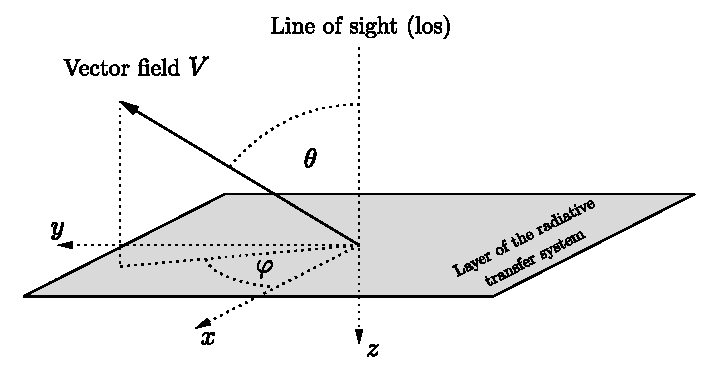
\includegraphics[width=0.8\textwidth]{figures/thesis/inclinationazimuth.pdf}
	\caption{Visualization of the definitions for the inclination and azimuth angles $\theta$ and $\varphi$.}
\end{figure}
\end{frame}

\section{Normalizing flows}
\begin{frame}[allowframebreaks]{Normalizing flows}
\framesubtitle{Why use normalizing flows for inversions?}
There are two main reasons to use normalizing flows for inversions:
\begin{enumerate}
\item Only simple atmospheric models can be inverted analytically. Therefore, one needs to resort to numerical methods, which are computationally demanding. Normalizing flows are - once trained - comparatively faster.
\item Numerical methods usually return a single solution to an inversion problem. Normalizing flow however return an entire probability density.
\end{enumerate}
\end{frame}

\begin{frame}[allowframebreaks]{Normalizing flows}
	\framesubtitle{What has been done yet using normalizing flows?}
Normalizing flows were introduced in 2015 by \cite{Rezende.21.05.2015} as a new solution to approximate posterior probability densities $p(\vect{x}|\vect{y})$.

\cite{DiazBaso.2022} applied normalizing flows to learn stellar atmospheric inversions using LTE and non-LTE models.

The thesis at hand comes in here to explore normalizing flows applied to learn the full Milne-Eddington inversion task (with magn. field parameters).
\end{frame}

\begin{frame}[allowframebreaks]{Normalizing flows}
\framesubtitle{How does a normalizing flow work?}
A flow is a generative model, which transforms a target probability density $p_{\vect{x}}(\vect{x})$ into a latent (base) probability density $p_{\vect{z}}(\vect{z})$.

Members $\vect{x}$ of the target probability density $p_{\vect{x}}(\vect{x})$ are optionally conditioned on data $\vect{y}$. (Sometimes $\vect{y} = \vect{M}(\vect{x})$).

\begin{figure}[h!]
	\centering
	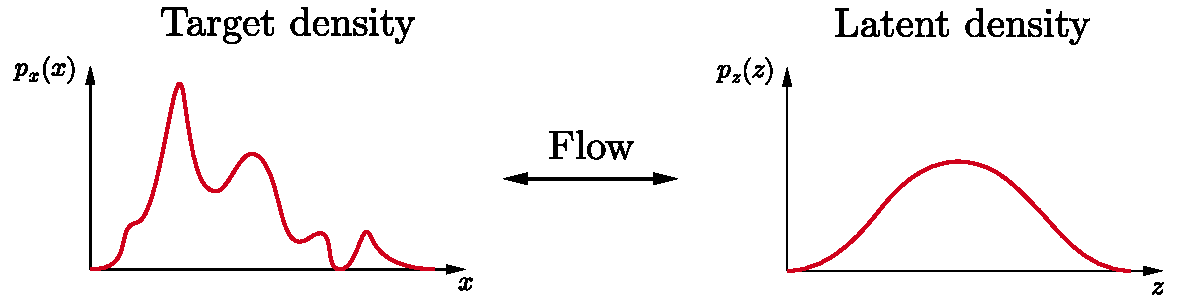
\includegraphics[width=0.9\textwidth]{figures/presentation/flowsimple.pdf}
	\caption{Simple illustration of the working principle of a normalizing flow.}
	\label{fig:flowsimple}
\end{figure}
\end{frame}


\begin{frame}[allowframebreaks]{Normalizing flows}
\vspace{-0.5cm}
\framesubtitle{Affine coupling layer normalizing flows}
\begin{figure}[h]
	\centering
	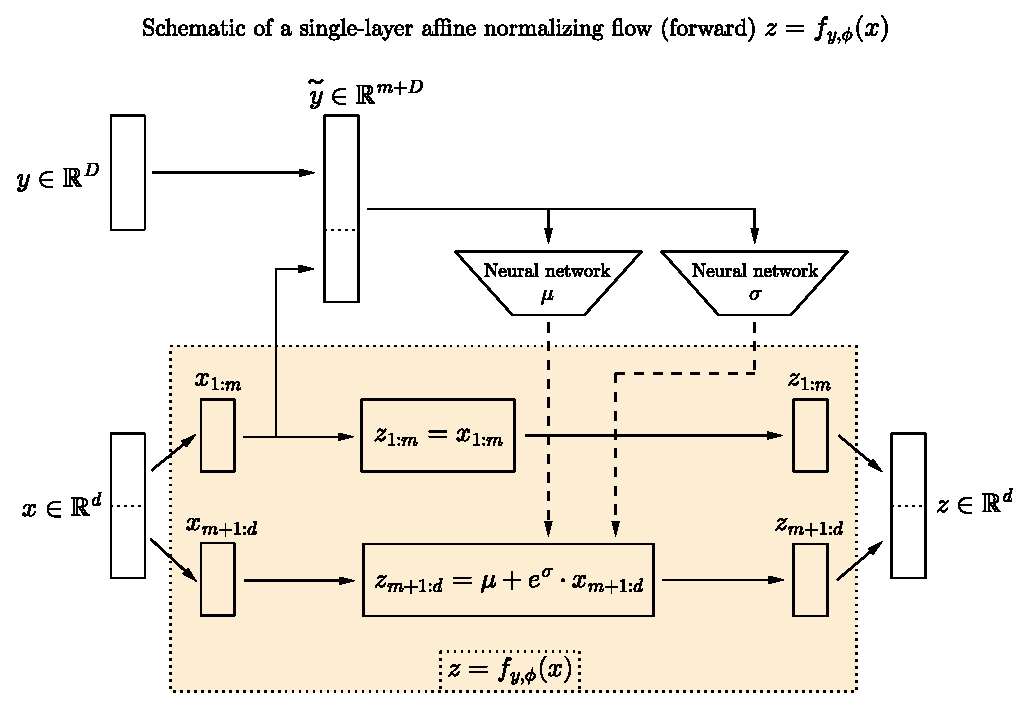
\includegraphics[width=0.8\textwidth]{figures/thesis/affinenormalizingflow_forward.pdf}
	\caption{Single-layer affine (coupling layer) normalizing flow (forward).}
	\label{fig:nflowaffine_forward}
\end{figure}
\end{frame}

\begin{frame}[allowframebreaks]{Normalizing flows}
	\vspace{-0.5cm}
	\framesubtitle{Affine coupling layer normalizing flows}
	\begin{figure}[h]
		\centering
		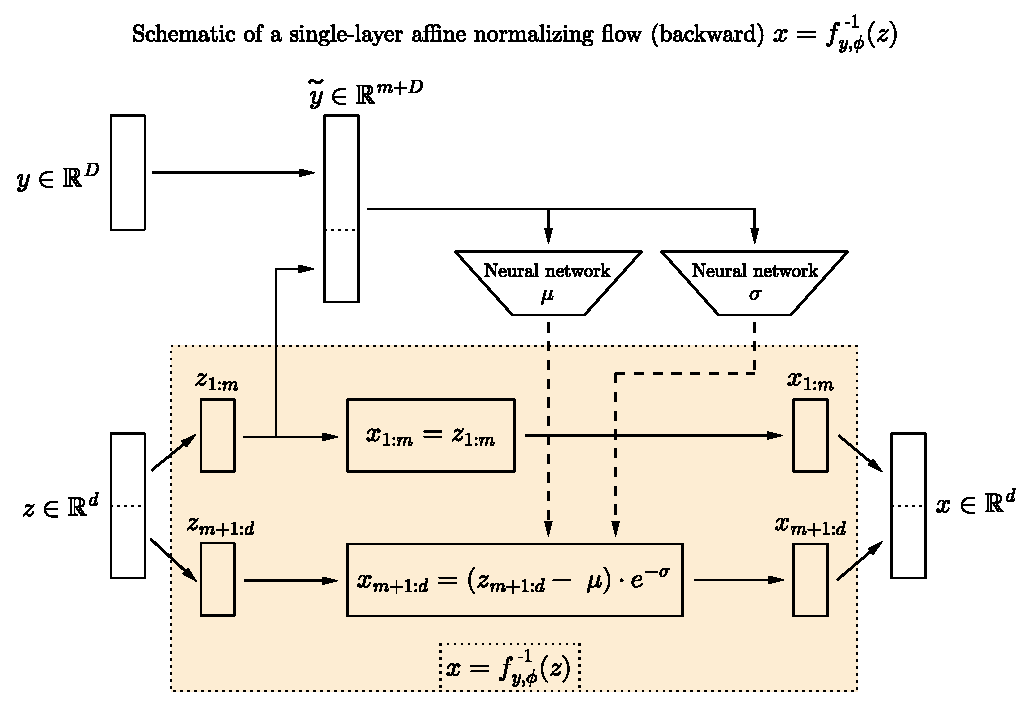
\includegraphics[width=0.8\textwidth]{figures/thesis/affinenormalizingflow_backward.pdf}
		\caption{Single-layer affine (coupling layer) normalizing flow (backward).}
		\label{fig:nflowaffine_backward}
	\end{figure}
\end{frame}

\begin{frame}[allowframebreaks]{Normalizing flows}
	\framesubtitle{Issues of affine coupling layer flows}
While simple to implement, affine coupling layer flows lack flexibility.

\cite[p.3]{Durkan.10.06.2019} note, that they especially struggle with modeling multimodal density functions.

Therefore, \cite[p.4]{Durkan.10.06.2019} suggest piecewise quadratic spline flows.

They are more flexible at modeling multimodal density functions, as \cref{fig:affinevsquadratic} shows.

\begin{figure}[h]
	\centering
	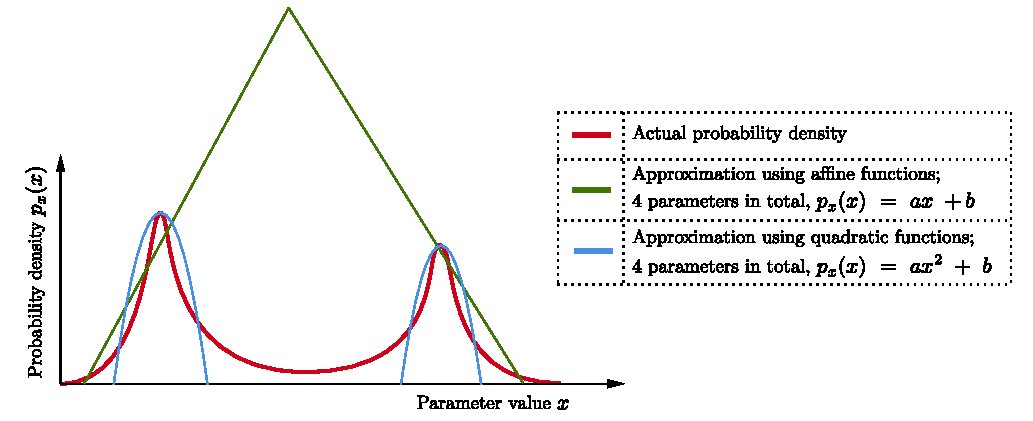
\includegraphics[width=\textwidth]{figures/presentation/affinevsquadratic.pdf}
	\caption{Approximating a probability density with affine or quadratic functions using the same amount of parameters in both cases.}
	\label{fig:affinevsquadratic}
\end{figure}
\end{frame}

\section{Results and discussion}
\begin{frame}[allowframebreaks]{Results and discussion}
\framesubtitle{General information about experiments}
The stellar atmospheric model for all of four presented experiments was the Milne-Eddington model. It extracts 9 atmospheric parameters from four Stokes profiles.

The experiments were performed on penumbra formation maps obtained by the space weather group at the Swedish Solar Telescope (SST).

This data contains a FOV of 550 by 600 pixels with four Stokes profiles consisting of 13 wavelength points each for each pixel.

The observations focus on the Fe I absorption line centered at $\lambda_0 = \SI{6302.4931}{\angstrom}$.

The Milne-Eddington model for the experiments can be specified as
\begin{gather}\small\begin{gathered}\label{model:Milne-Eddington_obs}
	\vect{M}:\mathbb{R}^9 \rightarrow \mathbb{R}^{52}, \quad \vect{x} = \begin{pmatrix}
		|\vect{B}| \\
		\theta \\
		\varphi \\
		v_{los} \\
		v_{dop} \\
		a \\
		\eta_0 \\
		S_0 \\
		S_1
	\end{pmatrix} \mapsto \vect{y} = \vect{M}(\vect{x}) = \begin{pmatrix}
		\vect{I}_{\lambda_{min}} \\
		\vdots \\
		\vect{I}_{\lambda_0} \\
		\vdots \\
		\vect{I}_{\lambda_{max}}
	\end{pmatrix},
 \end{gathered}\end{gather} where $\vect{I}_\lambda$ are the normalized Stokes parameters at wavelength $\lambda$.
\end{frame}

\begin{frame}[allowframebreaks]{Results and discussion}
\framesubtitle{Multiple map analysis: Experiment explanation} % Experiment 3
The penumbra formation dataset contains 16 frames. Frame 0 containing observational data $\hat{\matr{y}}$ was inverted using the Milne-Eddington algorithm, yielding corresponding atmospheric parameter data $\hat{\matr{x}}$.

A normalizing flow was trained on the data $\hat{\matr{x}}, \,\hat{\matr{y}}$ to map a 9-dimensional standard normal distribution to the distribution of atmospheric parameters.

Given an observation $\vect{y}$ (Stokes profiles of one pixel) and many samples $\vect{z} \sim \mathcal{N}(0,1)^9$ of a 9-dimensional standard distribution, one obtains densities for the nine atmospheric parameters.
\end{frame}

%\begin{frame}[allowframebreaks]{Results and discussion}
%	\vspace{-0.5cm}
%	\framesubtitle{Multiple map analysis: Experiment explanation} % Experiment 3
%	\begin{figure}[h]
%	\centering
%	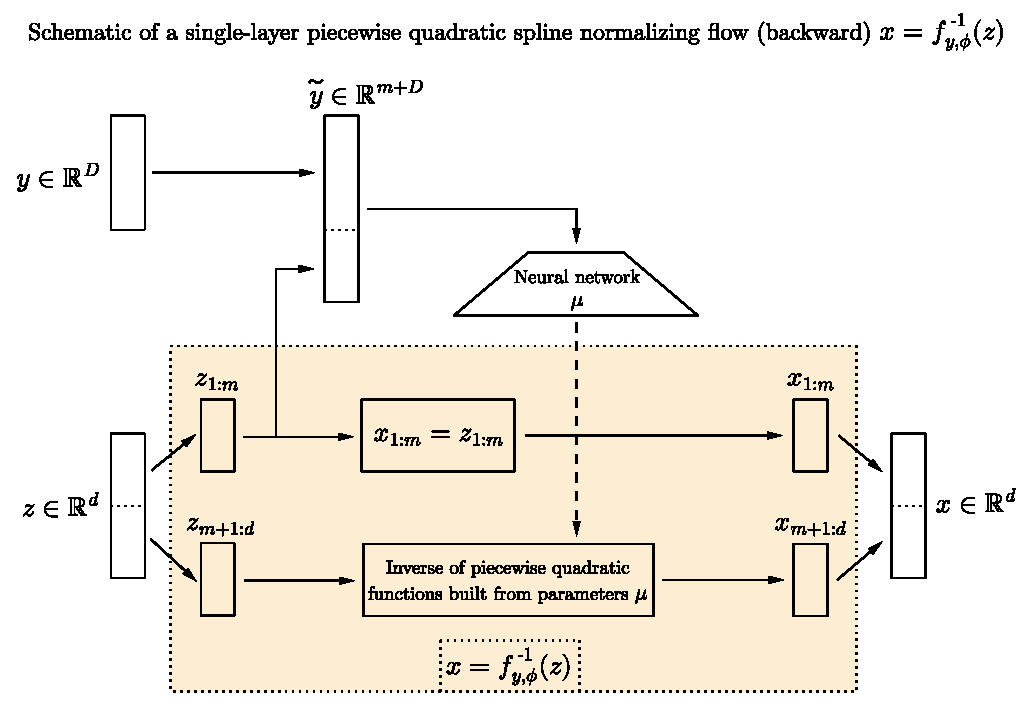
\includegraphics[width=0.8\textwidth]{figures/thesis/piecewisequadraticsplineflow_backward.pdf}
%	\caption{Single-layer piecewise quadratic spline (coupling layer) normalizing flow (backward).}
%	\label{fig:nflowquadratic_backwardb}
%\end{figure}
%\end{frame}

\begin{frame}[allowframebreaks]{Results and discussion}
\framesubtitle{Multiple map analysis: Experiment explanation} % Experiment 3
Figure \cref{fig:argmax} shows, how the solution to an inversion problem is obtained given the output of a normalizing flow for one pixel.

\begin{figure}[h!]
	\centering
	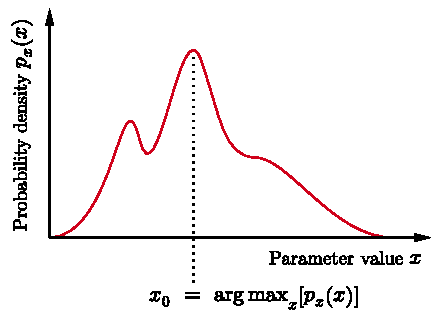
\includegraphics[width=4.3cm]{figures/thesis/argmax.pdf}
	\caption{Determining the solution of an inversion problem using normalizing flows. Suppose, $x \sim p_x(x)$ is the output of the normalizing flow. In order to get the most probable solution $x_0$ as given by the normalizing flow, one can take $x_0$ to be the argument of maximal probability of $p_x(x)$. 500 samples per atmospheric parameter were used in experiments.}
	\label{fig:argmax}
\end{figure}
\end{frame}

\begin{frame}[allowframebreaks]{Results and discussion}
	\framesubtitle{Multiple map analysis: Results} % Experiment 3
\begin{figure}[h!]
	\centering
	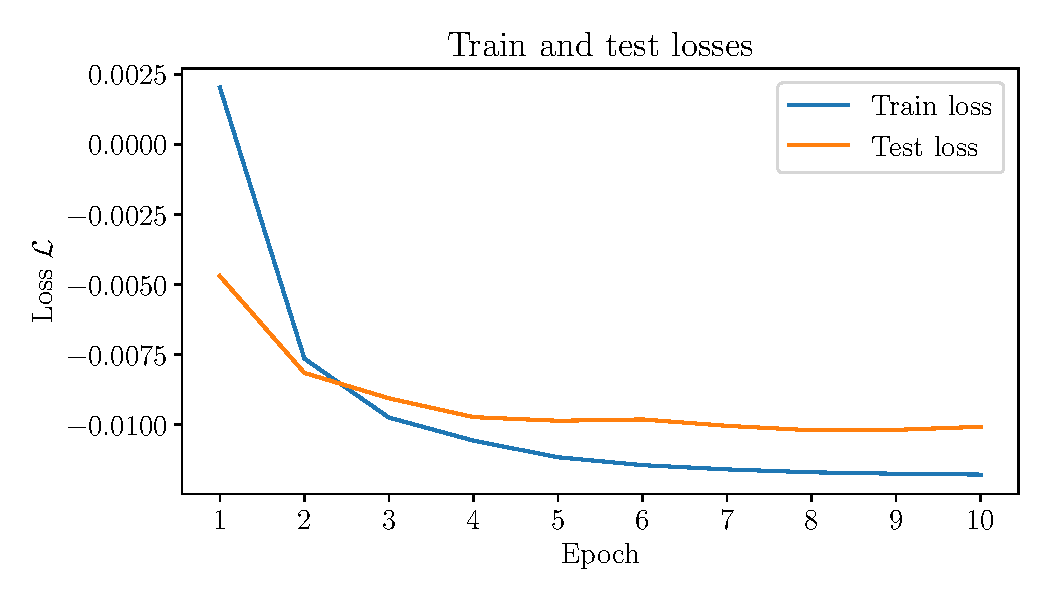
\includegraphics[width=8cm]{figures/thesis/nf-milne-eddington-example-2-loss-nflows-piecewisequadratic.pdf}
	\caption{Learning curve for multiple map analysis experiment.}
	\label{fig:nf-milne-eddington-example-2-loss-nflows-piecewisequadratic}
\end{figure}
\end{frame}

\begin{frame}[allowframebreaks]{Results and discussion}
	\framesubtitle{Multiple map analysis: Results} % Experiment 3
	\begin{figure}[h!]
		\centering
		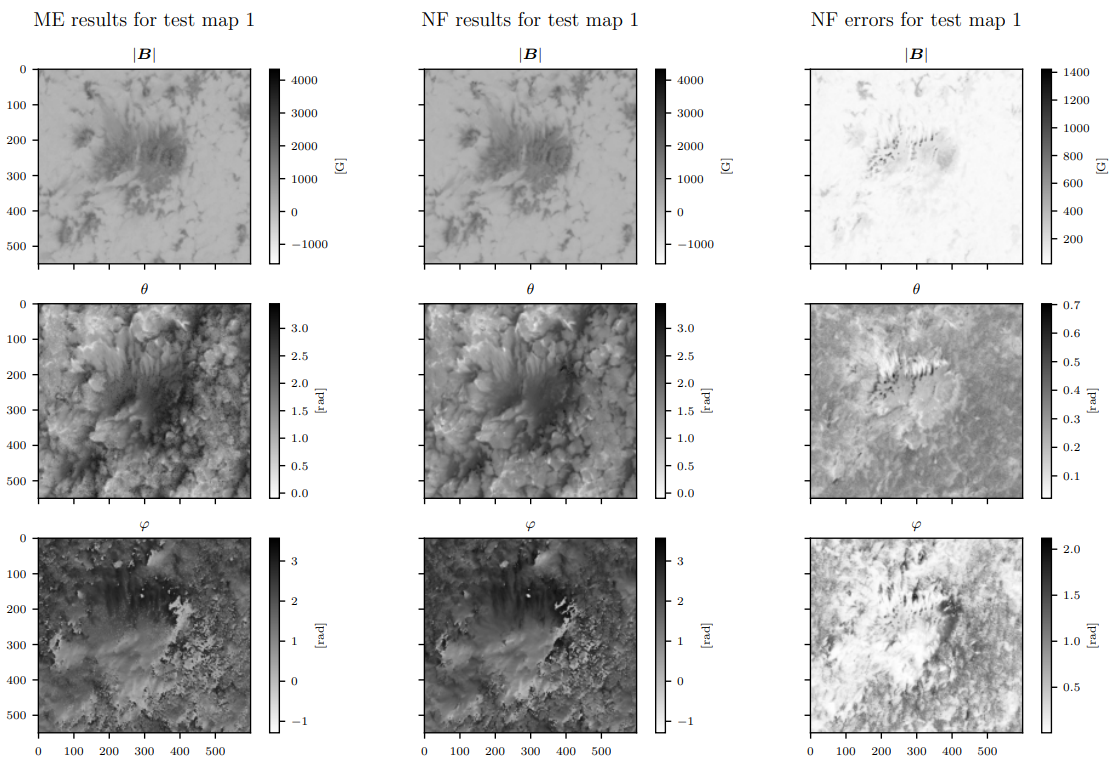
\includegraphics[width=8cm]{figures/presentation/exp3_fig1.png}
		\caption{Results for multiple map analysis experiment.}
		\label{fig:exp3_fig1}
	\end{figure}
\end{frame}

\begin{frame}[allowframebreaks]{Results and discussion}
\framesubtitle{Multiple map analysis: Results} % Experiment 3
There are three key points to take away from these results:
\begin{enumerate}
\item Train and test losses do not behave ideally, as they indicate slight overfitting.
\item Normalizing flows used for atmospheric inversions seem to have a tendency to smooth out edges, corners and sharp transitions: The ``smoothing property''.
\item Errors as calculated as standard deviations of the obtained probability densities for atmospheric parameters show expected behaviour for inclination and azimuth.
\end{enumerate}
\end{frame}

\begin{frame}[allowframebreaks]{Results and discussion}
\framesubtitle{Improving normalizing flow performance by enhancing the training dataset: Experiment explanation} % Experiment 5
This experiment consisted of successively increasing the size of the training dataset to see, whether the normalizing flow trained on it leads to ``better'' inversion results.

For this purpose, frame 0, frames 0 and 1 and frames 0, 1 and 2 of the penumbra formation dataset were used as training data (Stokes profiles $\hat{\matr{y}}$ with associated parameters $\hat{\matr{x}}$).

The three models were used to invert the last frame of the penumbra formation dataset.

Direct comparison to the Milne-Eddington inversion results for the same frame leads to an assessment of the results.
\end{frame}

\begin{frame}[allowframebreaks]{Results and discussion}
	\framesubtitle{Improving normalizing flow performance by enhancing the training dataset: Results} % Experiment 5
\begin{figure}[h]
	\centering
	\begin{subfigure}[t]{0.32\textwidth}
		\centering
		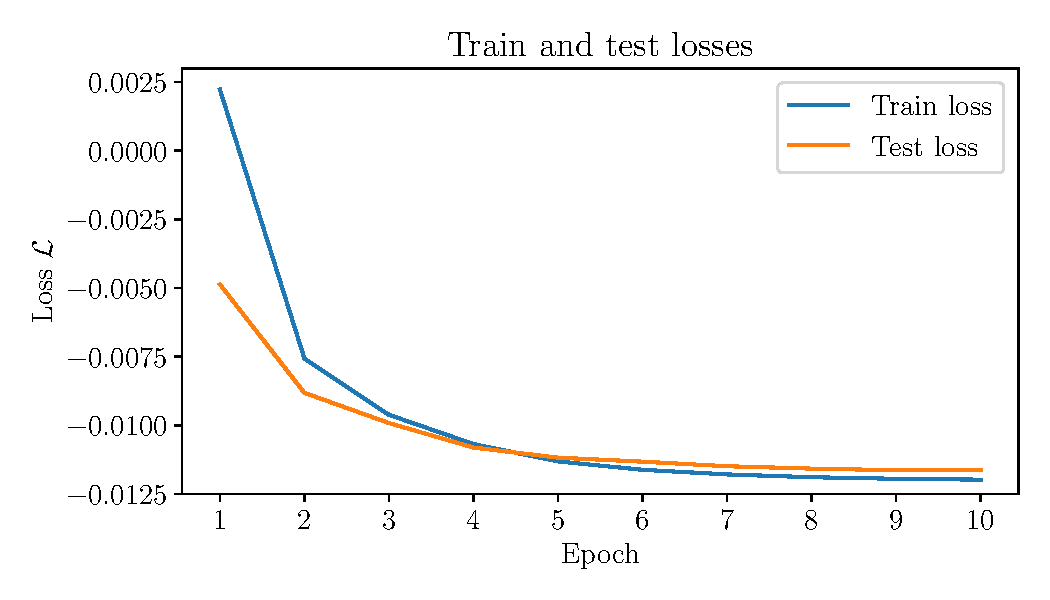
\includegraphics[width=\textwidth]{figures/thesis/nf-milne-eddington-example-5-loss-1train-nflows-piecewisequadratic.pdf}
		\caption{Normalizing flow trained on one frame.}
		\label{fig:nf-milne-eddington-example-5-loss-1train-nflows-piecewisequadratic}
	\end{subfigure}
	\hfill
	\begin{subfigure}[t]{0.32\textwidth}
		\centering
		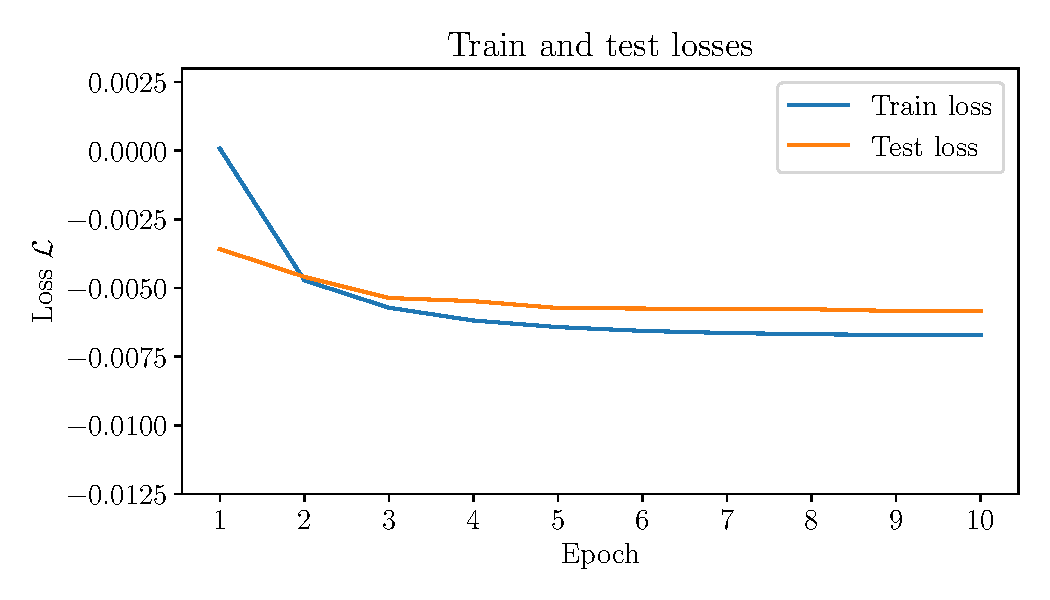
\includegraphics[width=\textwidth]{figures/thesis/nf-milne-eddington-example-5-loss-2train-nflows-piecewisequadratic.pdf}
		\caption{Normalizing flow trained on two frames.}
		\label{fig:nf-milne-eddington-example-5-loss-2train-nflows-piecewisequadratic}
	\end{subfigure}
	\hfill
	\begin{subfigure}[t]{0.32\textwidth}
		\centering
		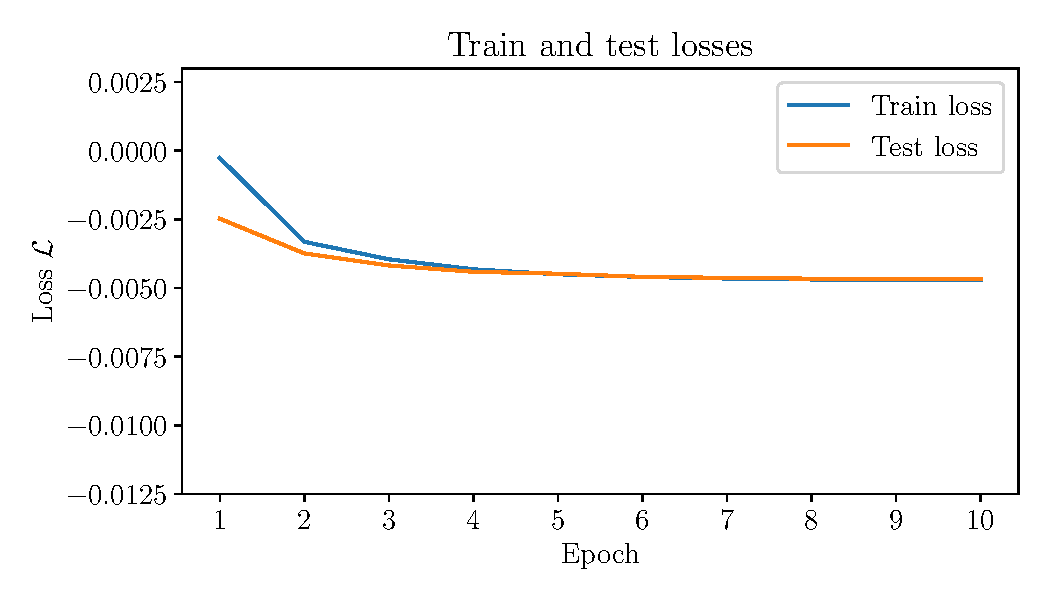
\includegraphics[width=\textwidth]{figures/thesis/nf-milne-eddington-example-5-loss-3train-nflows-piecewisequadratic.pdf}
		\caption{Normalizing flow trained on three frames.}
		\label{fig:nf-milne-eddington-example-5-loss-3train-nflows-piecewisequadratic}
	\end{subfigure}
	\caption{Train \& test losses for different sizes of train/test datasets.}
	\label{fig:nf-milne-eddington-example-5-loss-nflows-piecewisequadratic}
\end{figure}
\end{frame}

\begin{frame}[allowframebreaks]{Results and discussion}
	\framesubtitle{Improving normalizing flow performance by enhancing the training dataset: Results} % Experiment 5
	\vspace{-0.5cm}
\begin{figure}[h!]
	\centering
	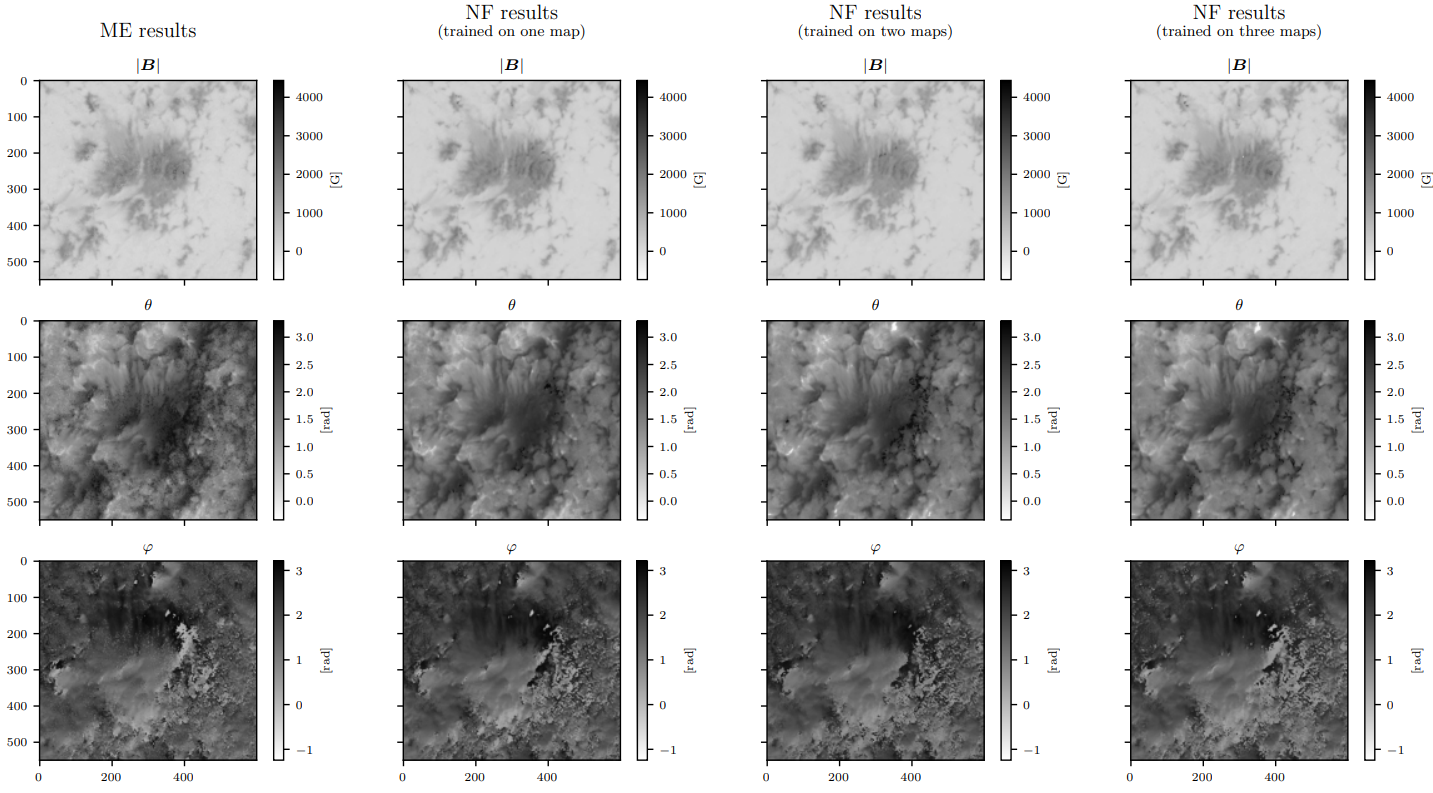
\includegraphics[width=\textwidth]{figures/presentation/exp5_fig1.png}
	\caption{Resulting inversion for improving normalizing flow performance by enhancement of the training dataset experiment.}
	\label{fig:exp5_fig1}
\end{figure}
\end{frame}

\begin{frame}[allowframebreaks]{Results and discussion}
	\framesubtitle{Improving normalizing flow performance by enhancing the training dataset: Results} % Experiment 5
\begin{figure}[h!]
	\centering
	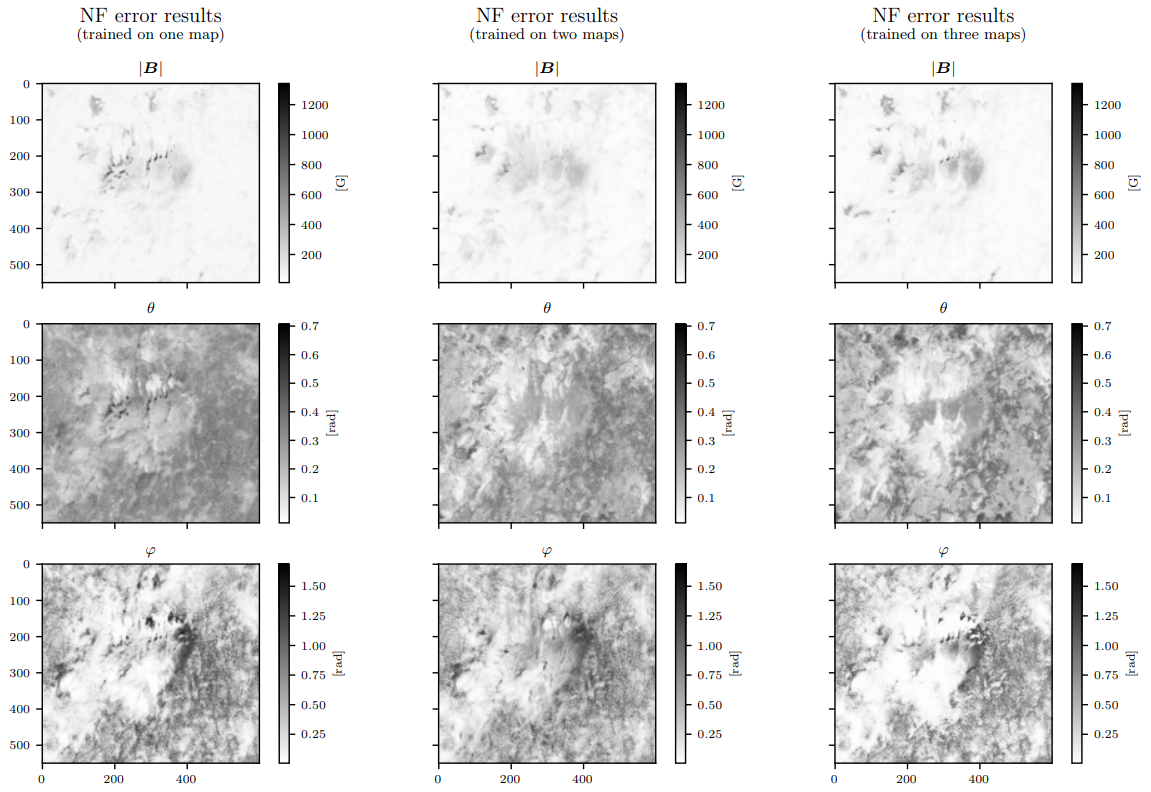
\includegraphics[width=8cm]{figures/presentation/exp5_fig2.png}
	\caption{Resulting inversion errors for improving normalizing flow performance by enhancement of the training dataset experiment.}
	\label{fig:exp5_fig2}
\end{figure}
\end{frame}

\begin{frame}[allowframebreaks]{Results and discussion}
	\framesubtitle{Improving normalizing flow performance by enhancing the training dataset: Results} % Experiment 5
\begin{figure}[h!] % Leave this picture here
	\centering
	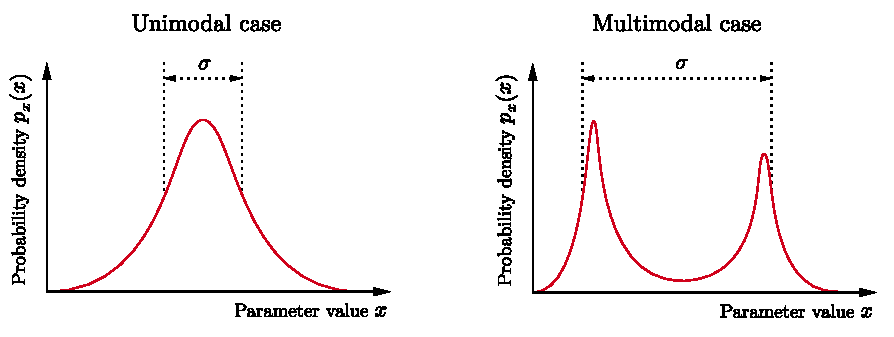
\includegraphics[width=0.8\textwidth]{figures/thesis/unimodal_multimodal.pdf}
	\caption{Visualization of the principle, that the standard variation $\sigma$ of a multimodal probability density is larger than that of an unimodal one, even if the multiple modes are sharply peaked - as long as the multiple peaks are sufficiently separated.}
	\label{fig:unimodal_multimodal}
\end{figure}
\end{frame}

\begin{frame}[allowframebreaks]{Results and discussion}
	\framesubtitle{Improving normalizing flow performance by enhancing the training dataset: Results} % Experiment 5
There are three key points to take away from these results:
\begin{enumerate}
	\item Train/test losses indicate, that overall performance is expected to increase with increasing size/variation of/in the training dataset.
	\item Overall uncertainties in normalizing flow inversions seem to decrease for increasing size in dataset. There are however areas, where errors increase.
	\item Generally speaking one can say, that increasing the amount of ``diversity'' in the training dataset, e.g. by taking into account more data for training, increases the overall performance of normalizing flows.
\end{enumerate}
\end{frame}

\section{Conclusions and outlook}
\begin{frame}[allowframebreaks]{Conclusions}
There are several conclusions to be drawn from the presented material:
\begin{enumerate}
\item Normalizing flows seem to be a useful tool with many applications.
%\item Experiments involving only synthetic data to train a normalizing flow could be promising.
%on were not successful (not shown here). Given enough computational resources however and simulating real-world effects in purely synthetic data, this could be a promising approach for further research.
\item Normalizing flows seem to provide reasonable results for inversions of the full Milne-Eddington model (LTE).
%Milne-Eddington inversions involving magnetic field parameters, if trained on real observational data and associated Milne-Eddington parameters. Further research on training normalizing flows on more complex atmospheric models (especially non-LTE models) would be interesting.
\item Increasing the size and hence variation in the training dataset seems to improve normalizing flow performance (captures more possible solutions).
%\item Normalizing flows seem promising for a simple LTE atmospheric models to infer atmospheric parameters.
%\item However, further research would be needed to quantify, if results are accurate enough to establish correlations of atmospheric parameters with solar eruptions.
\end{enumerate}% summarize conclusions and possible further work needed
\end{frame}

\begin{frame}[allowframebreaks]{Outlook}
	There are many possibilities for further research, e.g.:
	\begin{enumerate}
\item Build normalizing flow model solely trained on synthetic data. %It could be promising to train normalizing flows on synthetic data and apply the trained flow on real observational data. Real-world effects simulating influences of measurement processes on the data would have to be included in synthesizing data. 
\item Investigate performance of normalizing flows trained for more complex atmospheric models, e.g. SIR (LTE) or STiC (non-LTE). %Normalizing flows trained on observational data and associated Milne-Eddington (ME) parameters seem to perform well. The ME-model includes magnetic field parameters. It would be interesting to investigate the performance of normalizing flow trained on observational data and atmospheric parameter data obtained by a more complex atmospheric model, which also takes into account magnetic field parameters, e.g. SIR (LTE) or STiC (non-LTE).
\item Build normalizing flow model capable of inverting observations of any desired wavelength window. %It would also be a possibility to build a normalizing flow model trained on Stokes profiles for different wavelengths, such that observations of any desired wavelength window could be inverted by the flow.
\item Quantify, if normalizing flow results are accurate enough to identify possible precursors of solar eruptions.
	\end{enumerate}% summarize conclusions and possible further work needed
\end{frame}

\section*{Questions}
\begin{frame}[allowframebreaks]{Questions}
Thank you for your time and attention! Do you have any questions?
\end{frame}

\appendix

\section*{Literature}
\begin{frame}[allowframebreaks]{Literature}
\tiny
\bibliography{references}
\bibliographystyle{apalike}
\end{frame}

\section*{Appendix}
\begin{frame}[allowframebreaks]{Appendix}
	\framesubtitle{Why bother about inversions?}
	The ultimate goal of space weather is to identify triggers of solar flares and coronal mass ejections.
	
	Physical parameters in the Sun's atmosphere need to be known for that matter.
	
	Measurement directly within the solar atmosphere are not possible due to extreme environment; inference of atmospheric parameters from remote-sensing observations (spectral lines) is necessary.
\end{frame}

\begin{frame}[allowframebreaks]{Appendix}
	\framesubtitle{The Sun's characteristics}
	Object of investigation of the thesis is the Sun's atmosphere.
	
	The outer layers of the Sun are roughly divided into photosphere, chromosphere and corona.
	
	Depth of photosphere defined by optical depth, such that photons from below the photosphere cannot escape to space \cite[p.135]{Weigert.2006}.
	
	Interesting phenomena such as sunspots appear in the photosphere.
	
\end{frame}

\begin{frame}[allowframebreaks]{Appendix}
	\framesubtitle{The Sun's characteristics}
	\begin{figure}[h]
		\centering
		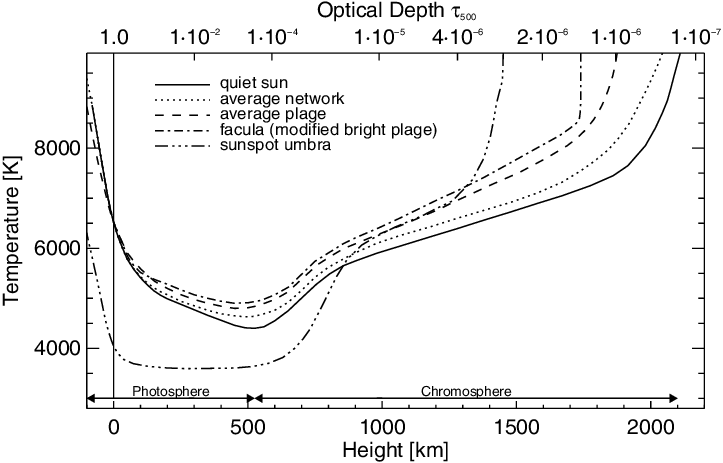
\includegraphics[width=0.7\textwidth]{figures/presentation/tempprofile.png}
		\caption{Temperature profile in the solar atmosphere. Figure taken from \cite[p.281]{Froehlich.2004}.}
	\end{figure}
\end{frame}


\begin{frame}[allowframebreaks]{Appendix}
	\framesubtitle{The Sun's characteristics}
	\begin{figure}[h]
		\centering
		\includegraphics[width=0.8\textwidth]{figures/thesis/Sunspots.pdf}
		\caption{Sunspots in the active region 10030, observed on July 15, 2002. Image credit: NASA Goddard Space Flight Center, \url{https://www.flickr.com/photos/gsfc/5510488494}, accessed on November 07, 2023. Adapted by the author.}
		\label{fig:Sunspots}
	\end{figure}
	
	Fully developed sunspots exhibit an umbra surrounded by a filament-like structure, the penumbra.
	
	A schematic visualization of a sunspot is given in the left panel of fig. 2; whereas the common bipolar sunspot arrangement is pictured in the right panel.
	
	\begin{figure}[h]
		\centering
		\begin{subfigure}{0.49\textwidth}
			\centering
			\includegraphics[width=0.7\textwidth]{figures/thesis/Sunspotsschematic.pdf}
		\end{subfigure}\hfill
		\begin{subfigure}{0.49\textwidth}
			\centering
			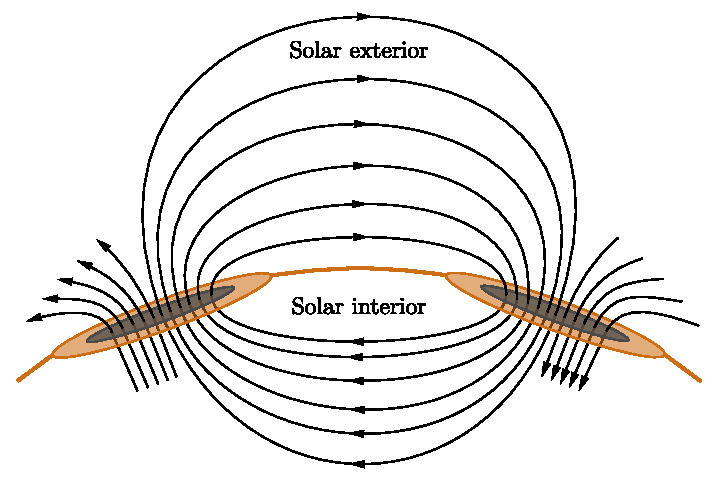
\includegraphics[width=0.7\textwidth]{figures/thesis/bipolarsunspots.pdf}
		\end{subfigure}
		\label{fig:sunspots}
		\caption{Schematic visualizations of sunspots. Note, that the magnetic field lines as drawn here could also be oriented exactly opposite.}
	\end{figure}
\end{frame}

\begin{frame}[allowframebreaks]{Appendix}
	\framesubtitle{Radiative transfer equation}
	\begin{columns} 
		% Column 1
		\begin{column}{.6\textwidth}
			Using \cref{fig:radiative-transfer-equation}, the radiative transfer equation can be derived to take the form
			\begin{equation}\label{eq:transportequationdiffform_opt_depth}
				\cos(\theta)\frac{\mathrm{d}I_\lambda(\tau^\prime_\lambda)}{\mathrm{d}\tau^\prime_\lambda} = I_\lambda(\tau^\prime_\lambda) - S_\lambda(\tau^\prime_\lambda).
			\end{equation} 
			
			The optical depth $\tau_{\lambda}^\prime$ is defined as $\mathrm{d}\tau_{\lambda}^\prime \doteq \alpha_\lambda\,\mathrm{d}z$, whereas $\tau_{\lambda}$ is the optical pathlength; $S_\lambda = j_\lambda/\alpha_\lambda$.
		\end{column}
		% Column 2    
		\begin{column}{.4\textwidth}
			\begin{figure}[h]
				\centering
				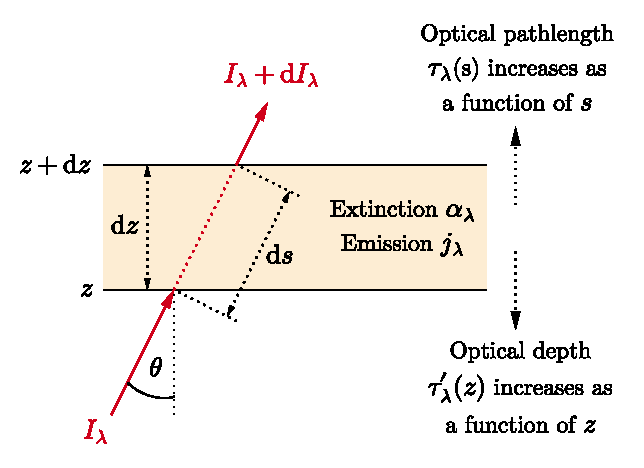
\includegraphics[width=\textwidth]{figures/thesis/radiative-transfer-equation.pdf}
				\caption{Illustration for the derivation of the radiative transfer equation. $[I_\lambda] = \si{\watt\per\steradian\per\cubic\meter}$ denotes the spectral radiance measured along a ray of inclination $\theta$ with respect to a horizontal plane in the coordinate system under consideration.}
				\label{fig:radiative-transfer-equation}
			\end{figure}
		\end{column}%
	\end{columns}
	
	\begin{columns}
		\begin{column}{0.59\textwidth}
			The formal solution of \cref{eq:transportequationdiffform_opt_depth} is given by integration from $\tau_\lambda^\prime$ to $\infty$ as
			\begin{gather}\footnotesize\begin{gathered}\label{eq:formaltransferequationoutward_depth}
					I^+_\lambda(\tau^\prime_\lambda, \theta) = \frac{1}{\cos(\theta)}\int_{\tau^\prime_\lambda}^{\infty} e^{\frac{\tau_\lambda^\prime - t}{\cos(\theta)}}S_\lambda(t)\,\mathrm{d}t,
			\end{gathered}\end{gather} known as outward spectral radiance (``intensity'').
			
			$S_\lambda(\tau_\lambda^\prime)$ is a source function describing photon emission at optical depth $\tau_\lambda^\prime$. 
			
			In thermodynamic equilibrium, $S_\lambda = B_\lambda$ with $B_\lambda$ the Planck function holds. 
		\end{column}
		
		\begin{column}{0.41\textwidth}
			\begin{figure}[h!]
				\centering
				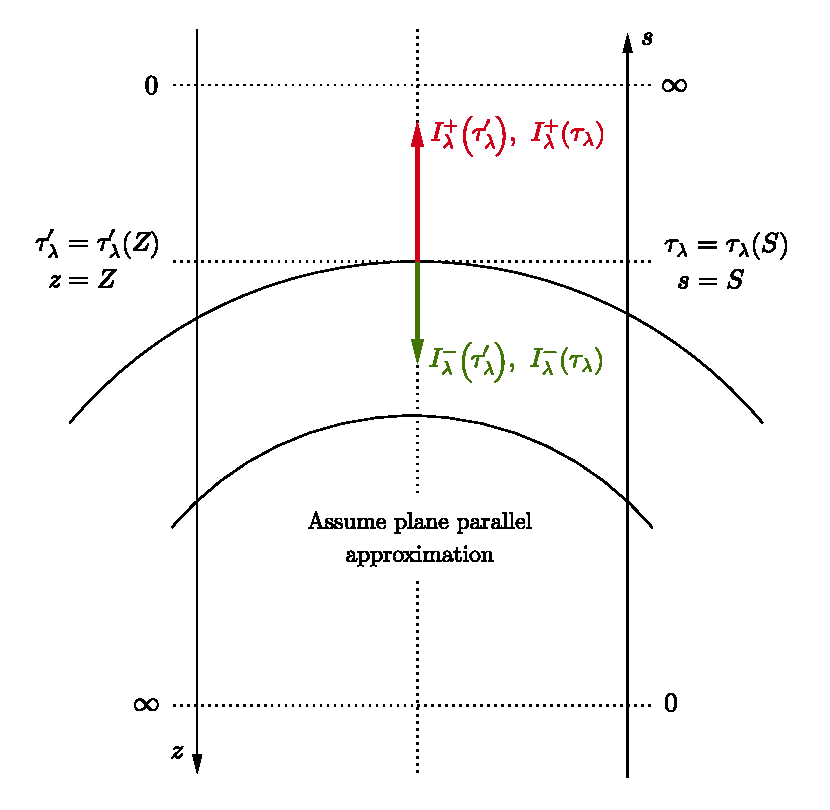
\includegraphics[width=\textwidth]{figures/thesis/outward-inward-radiation.pdf}
				\caption{Illustration of coordinate systems for optical pathlength $\tau_\lambda$ parametrized by $s$ and optical depth $\tau_\lambda^\prime$ parametrized by $z$.}
				\label{fig:outward-inward-radiation}
			\end{figure}
		\end{column}
	\end{columns}
\end{frame}

\begin{frame}[allowframebreaks]{Appendix}
	\framesubtitle{Radiative transfer equation}
	\begin{columns}
		\begin{column}{0.39\textwidth}
			In order to build an atmospheric model for a stellar atmosphere, radiative transfer is needed.
			
			The propagation of electromagnetic radiation through matter is described by the radiative transfer equation.
		\end{column}
		\begin{column}{0.6\textwidth}
			\begin{figure}[h]
				\centering
				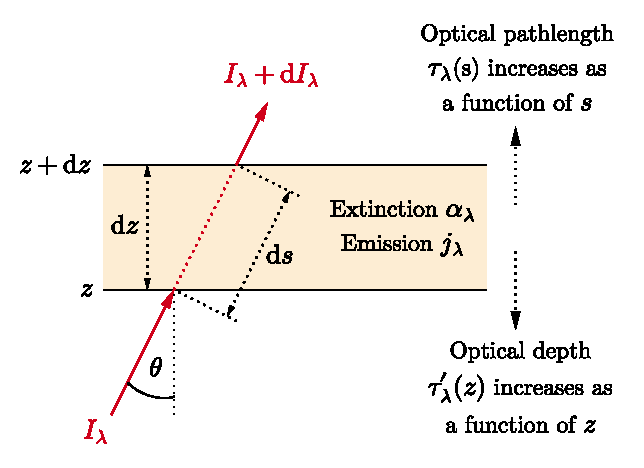
\includegraphics[width=\textwidth]{figures/thesis/radiative-transfer-equation.pdf}
				\caption{Illustration for the derivation of the radiative transfer equation. $[I_\lambda] = \si{\watt\per\steradian\per\cubic\meter}$ denotes the spectral radiance measured along a ray of inclination $\theta$ with respect to a horizontal plane in the coordinate system under consideration.}
			\end{figure}
		\end{column}
	\end{columns}
\end{frame}


\begin{frame}[allowframebreaks]{Appendix}
	\framesubtitle{Zeeman effect}
	\begin{columns}
		\begin{column}{0.49\textwidth}
			A radiative transfer system subject to a strong external magnetic field $\vect{B}$ will exhibit splitting of an absorption/emission line into several lines.
			
			This effect is known as the Zeeman effect and allows for inference of magnetic field strength.
			
			The ``distance'' between split energy levels is a function of magnetic field strength.
		\end{column}
		\begin{column}{0.49\textwidth}
			\begin{figure}[h]
				\centering
				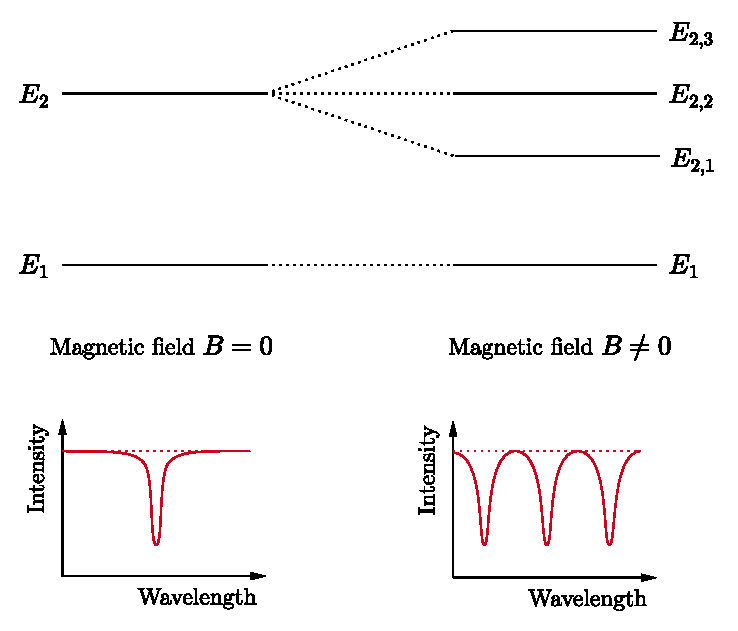
\includegraphics[width=\textwidth]{figures/thesis/zeemaneffect.pdf}
				\caption{Visualization of the Zeeman effect. Due to coupling of the magnetic moment of electrons with the external magnetic field, energy levels split into several sub-levels.}
				\label{fig:zeemaneffect}
			\end{figure}
		\end{column}
	\end{columns}
\end{frame}

\begin{frame}[allowframebreaks]{Appendix}
	\framesubtitle{Stokes parameters and Stokes vector}
	\begin{columns}
		\begin{column}{0.6\textwidth}
			The Stokes parameters $I_\lambda$, $Q_\lambda$, $U_\lambda$ and $V_\lambda$ contain information about the polarization properties of electromagnetic waves.
			
			The Stokes vector $\vect{I}_\lambda = (I_\lambda, Q_\lambda, U_\lambda, V_\lambda)^\top$ contains all four Stokes parameters.
			
			Values of the Stokes parameters in dependence of wavelength $\lambda$ are called Stokes profiles. They can be used to infer physical parameters of a radiative transfer system from observations.
		\end{column}
		\begin{column}{0.4\textwidth}
			\begin{figure}[h]
				\centering
				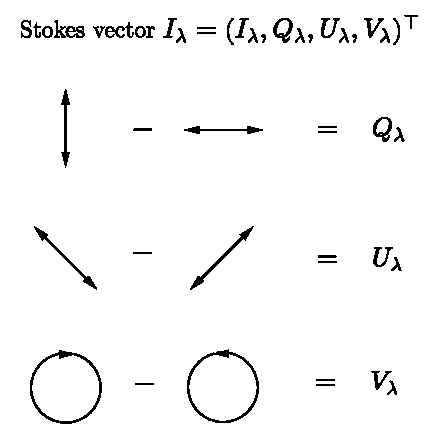
\includegraphics[width=\textwidth]{figures/thesis/stokesvector.pdf}
				\caption{Meaning of the four Stokes parameters for an electromagn. wave propagating towards the observer. Figure inspired by \cite[p.17]{DeglInnocenti.2005}.}
				\label{fig:stokesvector}
			\end{figure}
		\end{column}
	\end{columns}
\end{frame}

\begin{frame}[allowframebreaks]{Appendix}
	\framesubtitle{Generalized radiative transfer equation}
	In order to describe the change in all four Stokes parameters with optical depth, one needs to generalize the radiative transfer equation.
	
	The generalized radiative transfer equation encompasses all information about how different atmospheric parameters change with respect to optical depth; \cite[p.150]{delToroIniesta.2003} give it as \begin{equation}
		\frac{\mathrm{d}\vect{I}_\lambda(\tau_\lambda^\prime)}{\mathrm{d}\tau_\lambda^\prime} = \matr{K}_\lambda(\tau_\lambda^\prime)\left[\vect{I}_\lambda(\tau_\lambda^\prime)-\vect{S}_\lambda(\tau_\lambda^\prime)\right],
	\end{equation}
	were $\matr{K}_\lambda$ is the propagation matrix and $\vect{S}_\lambda(\tau_\lambda^\prime) = S_\lambda(\tau_\lambda^\prime)(1,0,0,0)^\top$ is the generalized source function.
\end{frame}

\begin{frame}[allowframebreaks]{Appendix}
	\framesubtitle{Spectral line formation}
	The Eddington-Barbier approximation provides a means to qualitatively understand spectral line formation.
	
	It is obtained as \begin{equation}
		I_\lambda^+(\tau_\lambda^\prime=0, \theta=0) \approx S_\lambda(\tau_\lambda^\prime = 1)
	\end{equation} by $S_\lambda(\tau_\lambda^\prime)$ as a power series in $\tau_\lambda^\prime$ and truncating terms of order $\mathcal{O}(\cos(\theta)^2)$ and higher.
	
	Essentially it says, that the intensity $I_\lambda^+$ perpendicular to the system's surface as measured by an observer outside the system is roughly given by the source function at optical depth $\tau_\lambda^\prime = 1$.
	
	\newpage
	\begin{columns}
		\begin{column}{0.45\textwidth}
			Eddington-Barbier relation: $I_\lambda^+(\tau_\lambda^\prime=0) \approx S_\lambda(\tau_\lambda^\prime=1)$.
			
			Assumptions:
			\begin{enumerate}
				\item Extinction coefficient $\alpha_\lambda$ independent of depth $z$; hence $\tau_\lambda^\prime(Z) = \int_{0}^Z\alpha_\lambda\,\mathrm{d}z = \alpha_\lambda Z$ holds.
				\item Source function $S_\lambda$ independent of wavelength $\lambda$ and affine in $z$, i.e. $S_\lambda = S = S_0 + S_1z$.
			\end{enumerate}
		\end{column}
		
		\begin{column}{0.55\textwidth}
			\begin{figure}[h]
				\centering
				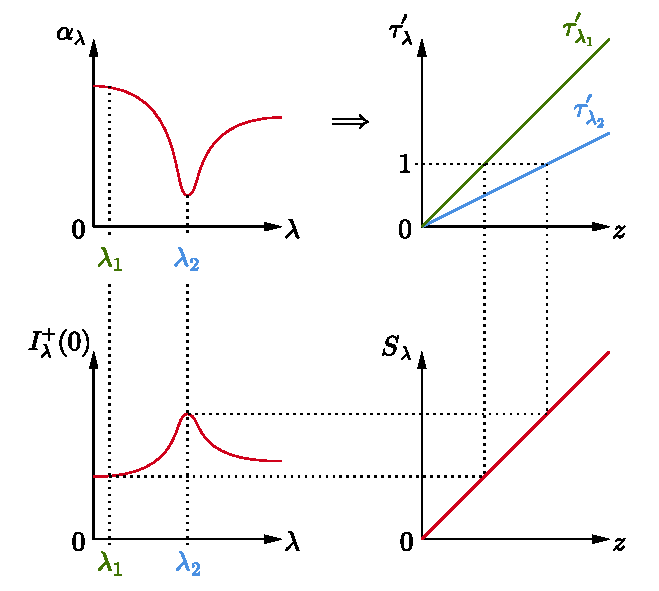
\includegraphics[width=\textwidth]{figures/thesis/spectrallineformation.pdf}
				\caption{Illustration of a spectral line formation using the Eddington-Barbier relation. Figure inspired by \cite[p.38]{Rutten.2015}.}
				\label{fig:spectrallineformation}
			\end{figure}
		\end{column}
	\end{columns}
\end{frame}

\begin{frame}[allowframebreaks]{Appendix}
	\framesubtitle{Generalized radiative transfer equation}
	The radiative transfer equation can be generalized to encompass information about the full Stokes vector $\vect{I}_\lambda$.
	
	The generalized radiative transfer equation is given as \begin{equation}\label{eq:generalizedradtransfereq}
		\frac{\mathrm{d}\vect{I}_\lambda(\tau_\lambda^\prime)}{\mathrm{d}\tau_\lambda^\prime} = \matr{K}_\lambda(\tau_\lambda^\prime)\left[\vect{I}_\lambda(\tau_\lambda^\prime)-\vect{S}_\lambda(\tau_\lambda^\prime)\right],
	\end{equation}
	were $\matr{K}_\lambda$ is the propagation matrix and $\vect{S}_\lambda(\tau_\lambda^\prime) = S_\lambda(\tau_\lambda^\prime)(1,0,0,0)^\top$ is the generalized source function \cite[p.150]{delToroIniesta.2003}.
	
	The propagation matrix $\matr{K}_\lambda$ encompasses all information about how the different atmospheric parameters affect the development of $\vect{I}_\lambda$ as a function of optical depth and wavelength.
	
	\newpage
	
	The general formal solution to \cref{eq:generalizedradtransfereq} is derived to be \begin{align}\label{eq:general_sol_gen_rad_transf_eq}\begin{aligned}
			\vect{I}_\lambda(\tau_\lambda^\prime) = \matr{P}\left(\tau_\lambda^\prime,\infty\right)\vect{I}_\lambda(\infty)  -\int_{\infty}^{\tau_\lambda^\prime}\matr{P}\left(\tau_\lambda^\prime,t\right)\matr{K}_\lambda(t)\vect{S}_\lambda(t)\,\mathrm{d}t,
	\end{aligned}\end{align}
	where $\matr{P}(\kappa, \kappa^\prime)$ is the so-called evolution operator giving the evolution of the homogeneous part from a point $\kappa^\prime$ to $\kappa$.
	
	At $\tau_\lambda^\prime=0$, i.e. at the position of an observer outside the radiative transfer system, the solution reduces to \begin{equation}\label{eq:gen_rad_trans_eqn_to_solve}
		\vect{I}_\lambda(\tau_\lambda^\prime = 0) = \int_{0}^\infty \matr{P}(0,t)\matr{K}_\lambda(t)\vect{S}_\lambda(t)\,\mathrm{d}t.
	\end{equation}
\end{frame}

\begin{frame}[allowframebreaks]{Appendix}
	\framesubtitle{Milne-Eddington approximation}
	
	\cite[p.411]{DeglInnocenti.2005} gives three assumptions pertaining to the Milne-Eddington approximations:
	\begin{enumerate}
		\item The radiative transfer system is assumed to be of a plane parallel nature and in a local thermodynamic equilibrium.
		\item All parameters relevant to spectral line formation are required to be independent of all measures of height within the system.
		\item The source function is required to be an affine function of the continuum optical depth.
	\end{enumerate}
	
\end{frame}
\begin{frame}[allowframebreaks]{Appendix}
	\framesubtitle{Milne-Eddington approximation}
	
	Implementing these assumptions as simplifications to \cref{eq:gen_rad_trans_eqn_to_solve}, one arrives as \begin{equation}
		\vect{I}_\lambda(\tau_\lambda^\prime=0) = \vect{S}_{\lambda,0} - \matr{K}_{\lambda,0}^{-1}\vect{S}_{\lambda,1}
	\end{equation} for the Milne-Eddington solution.
	
	By assumption 1., $\matr{K}_{\lambda,0}$ is the isotropically constant propagation matrix at wavelength $\lambda$.
	
	By assumption 2., the source function vector $\vect{S}_\lambda$ is given by $\vect{S}_\lambda(\tau_\lambda^\prime) = \vect{S}_{\lambda,0} + \tau_\lambda^\prime \vect{S}_{\lambda,1}$.
	
	By assumption 1., $\vect{S}_{\lambda,0}$ and $\vect{S}_{\lambda,1}$ are connected to the Planck function $B_\lambda(T)$ as $\vect{S}_{\lambda,0} = B_\lambda(T)(1,0,0,0)^\top = (S_0,0,0,0)^\top$ and $\vect{S}_{\lambda,1} = B_\lambda(T)\beta(1,0,0,0)^\top = (S_1,0,0,0)^\top$, $\beta \in \mathbb{R}$.
\end{frame}

\begin{frame}[allowframebreaks]{Appendix}
	\vspace{-0.5cm}
	\framesubtitle{Milne-Eddington (ME) model}
	\begin{table}[h]
		\centering
		\fontsize{7.5}{10}\selectfont % Set the custom font size (8pt with 10pt leading)
		\begin{tabularx}{\textwidth}{|c|X|}
			\hline
			\textbf{Parameter} & \textbf{Explanation} \\
			\hline\hline
			$|\vect{B}|$ & Magnitude of the magnetic field vector. \\
			\hline
			$\theta$ & Inclination value of the magnetic field vector. $\theta=0$ means orientation of the magnetic field towards the observer, $\theta = \pi$ away from the observer.\\
			\hline
			$\varphi$ & Azimuth value of the magnetic field vector. $\varphi=0$ means orientation of the magnetic field towards solar north, $\varphi = \pi/2$ towards solar east.\\
			\hline
			$v_{los}$ & Line of sight velocity of emitting/absorbing matter. \\
			\hline
			$v_{dop}$ & Doppler velocity corresponding to the Doppler broadening $\Delta \lambda_D = v_{dop}\lambda / c$ of spectral lines. \\
			\hline
			$a$ & Damping parameter affecting the spectral line shape. The damping is strong for high values of $a$ and vice versa. \\
			\hline
			$\eta_0$ & Line strength parameter for spectral lines. A spectral line is highly pronounced relative to the continuum for high values of $\eta_0$ and vice versa. \\
			\hline
			$S_0$ & Shift parameter for the source function as an affine function of optical depth. \\
			\hline
			$S_1$ & Scale parameter for the source function as an affine function of optical depth. \\
			\hline
		\end{tabularx}
		\caption{Summary of the nine Milne-Eddington atmospheric parameters.}
		\label{tab:paramsummary}
	\end{table}
\end{frame}

\begin{frame}[allowframebreaks]{Appendix}
	\framesubtitle{Neural networks}
	The basic building block of neural networks is given by the perceptron \cite[pp.338-342]{Raschka.2022}.
	
	The perceptron is constructed somewhat analogous to a neuron in the human brain, as \cref{fig:neuronperceptron} shows.
	
	A deep neural network can be build by multiple layers of interconnected perceptrons.
	
	The perceptron as seen in the right panel of \cref{fig:neuronperceptron} has an input $\vect{x} = (x_1,\dots,x_d)^\top$ and an output $\bar{x}$.
	
	The quantity $s = b + \sum_{i=1}^d x_i\phi_i$ is calculated with weights $\phi_i$ and a bias $b$.
	
	The sum $s$ is passed through an suitable (non-linear) activation function $a:\mathbb{R}\rightarrow \mathbb{R}, \, s \mapsto a(s)$, which generates the output value $\bar{x}$.
	
\end{frame}
\begin{frame}[allowframebreaks]{Appendix}
	\framesubtitle{Neural networks}
	
	\begin{figure}[h]
		\centering
		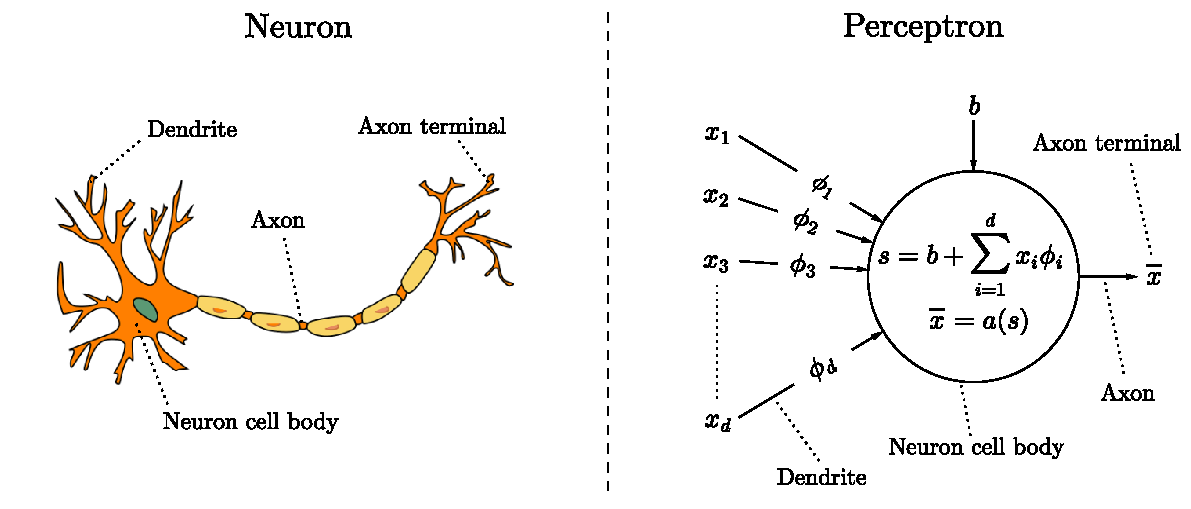
\includegraphics[width=0.9\textwidth]{figures/thesis/neuronperceptron.pdf}
		\caption{Visualization of the similarities between a human brain neuron and a perceptron. Image credit for image in left panel: Clker-Free-Vector-Images, \url{https://www.needpix.com/photo/170704/}, accessed on January 02, 2024. Adapted by the author.}
		\label{fig:neuronperceptron}
	\end{figure}
	
\end{frame}
\begin{frame}[allowframebreaks]{Appendix}
	\framesubtitle{Neural networks}
	
	In order for a neural network to learn anything, it has to be conditioned by data, whose interpretation is known. This process is known as training.
	
	Training requires a mathematical framework allowing for optimization of the network parameters (weights and biases).
	
	A loss function $\mathcal{L}_{\vect{\phi}}$ depending on network parameters $\vect{\phi}$ is defined, which is a measure for the discrepancy between network output and true value(s) of the training data.
	
	Neural networks are commonly trained by gradient descent as visualized in \cref{fig:gradientdescent}.
	
\end{frame}
\begin{frame}[allowframebreaks]{Appendix}
	\framesubtitle{Neural networks}
	
	\begin{columns}
		\begin{column}{0.6\textwidth}
			The training process works as follows:
			\begin{enumerate}
				\item Take a start value $\vect{\phi}_0$ and calculate the value of the loss function $\mathcal{L}_{\vect{\phi}_0}$ at this point.
				\item Update the weights $\vect{\phi}_{i}$ according to the rule \begin{equation}
					\vect{\phi}_{i+1} = \vect{\phi}_{i} - \gamma \vect{\nabla}_{\vect{\phi}}\mathcal{L}_{\vect{\phi}_i}
				\end{equation} for $i \in \mathbb{N}$ individual steps and $\gamma \in \mathbb{R}$ a suitable step size as long as $\epsilon \leq |\mathcal{L}_{\vect{\phi}_{i+1}}-\mathcal{L}_{\vect{\phi}_{i}}|$ holds for $\epsilon \in \mathbb{R}$ an accuracy threshold.
				\item Terminate, if $\epsilon > |\mathcal{L}_{\vect{\phi}_{i+1}}-\mathcal{L}_{\vect{\phi}_{i}}|$.
			\end{enumerate}
		\end{column}
		\begin{column}{0.4\textwidth}
			\begin{figure}[h]
				\centering
				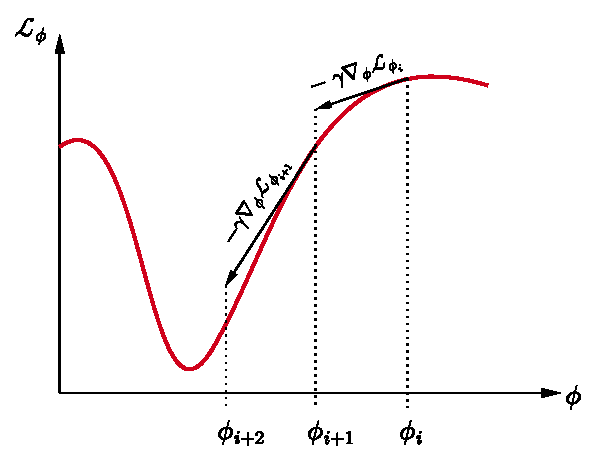
\includegraphics[width=\textwidth]{figures/thesis/gradientdescent.pdf}
				\caption{Visualization of a gradient descent routine.}
				\label{fig:gradientdescent}
			\end{figure}
		\end{column}
	\end{columns}
	
\end{frame}

\begin{frame}[allowframebreaks]{Appendix}
	\framesubtitle{Learning curves}
	\begin{figure}[h]
		\centering
		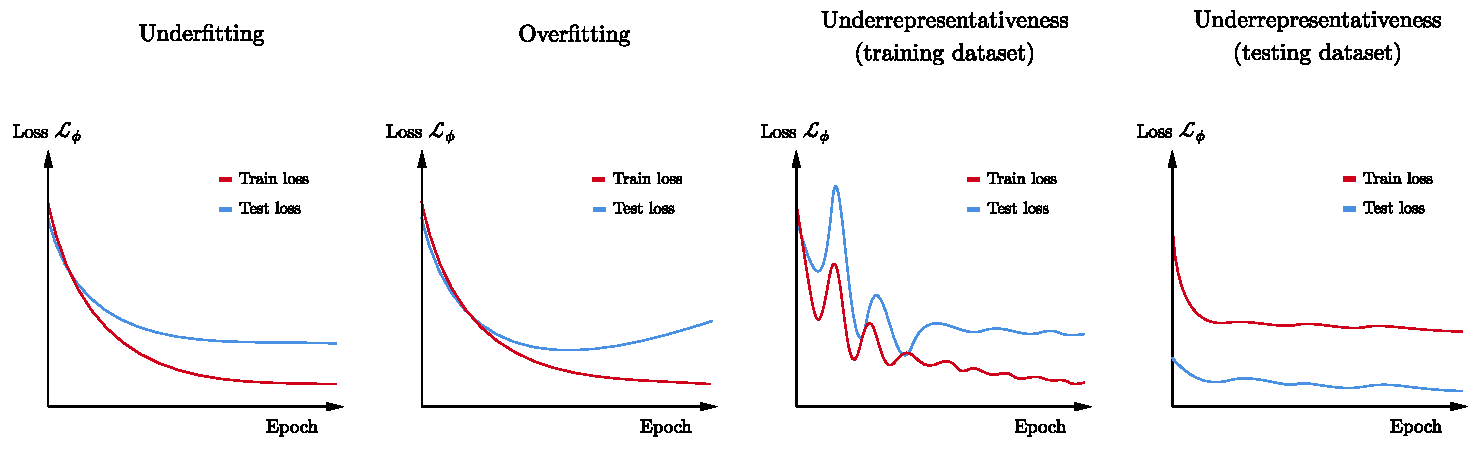
\includegraphics[width=\textwidth]{figures/thesis/learningcurves.pdf}
		\caption{Examples for the four basic cases of non-ideal model performance. Sketches inspired by Jason Brownlee, \url{https://machinelearningmastery.com/learning-curves-for-diagnosing-machine-learning-model-performance/}, accessed on December 18, 2023.}
		\label{fig:learningcurves}
	\end{figure}
	
	\begin{figure}[h]
		\centering
		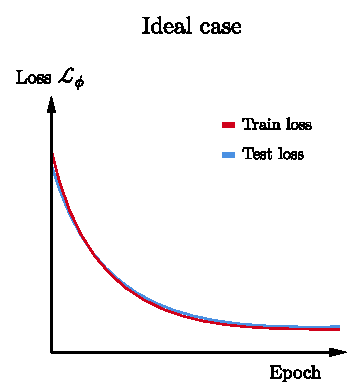
\includegraphics[width=5.5cm]{figures/thesis/ideallearningcurve.pdf}
		\caption{Example of an ideal learning curve.}
		\label{fig:ideallearningcurve}
	\end{figure}
	
\end{frame}

\begin{frame}[allowframebreaks]{Appendix}
	\framesubtitle{Flows as deep generative models}
	A so-called flow (or normalizing flow) is a type of generative model, as e.g. GAN's and VAE's are \cite{weng2018flow}.
	
	The principle of a flow is visualized in \cref{fig:Flow}.
	
	A flow is called a normalizing flow, if the latent distribution $\vect{z}\sim p_{\vect{z}}(\vect{z})$ is chosen as a standard normal distribution.
	
	An arbitrary probability density $p_{\vect{x}}(\vect{x})$ is mapped to the latent density $p_{\vect{z}}(\vect{z})$ by the diffeomorphic flow $\vect{f}_{\vect{\phi}}(\vect{x})$.
	
	Flows can be trained by the negative log-likelihood, which can be exactly calculated using the specific transformation $\vect{f}_{\vect{\phi}}$ used as a flow in combination with the change of variable theorem.
	
	\begin{figure}[h!]
		\centering
		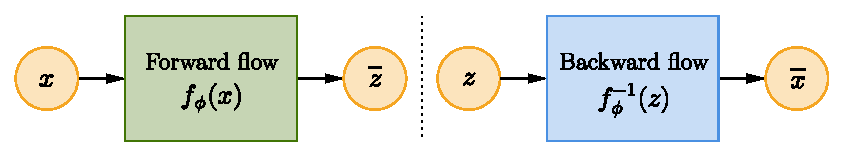
\includegraphics[width=0.9\textwidth]{figures/thesis/Flow.pdf}
		\caption{Working principle of a flow-based generative model. Figure inspired by \cite{weng2018flow}.}
		\label{fig:Flow}
	\end{figure}
\end{frame}

\begin{frame}[allowframebreaks]{Appendix}
	\framesubtitle{How does a normalizing flow work?}
	\begin{figure}[h]
		\centering
		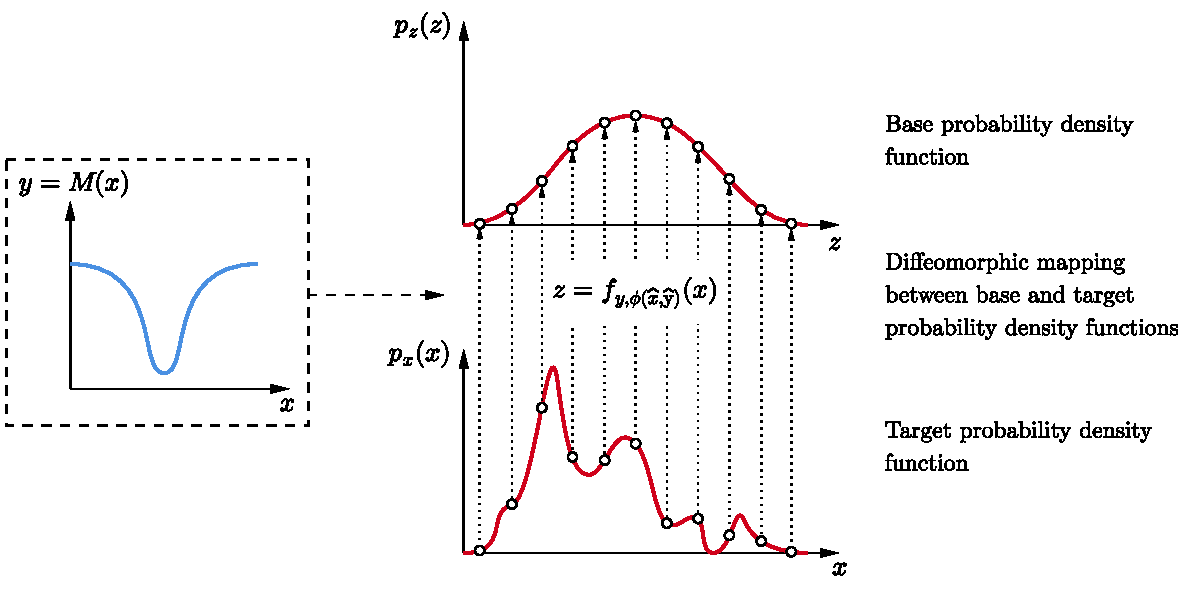
\includegraphics[width=0.8\textwidth]{figures/thesis/normflowconditional.pdf}
		\caption{Conceptual principle of a conditional normalizing flow $\vect{z} = \vect{f}_{\vect{y},\vect{\phi}(\hat{\matr{x}},\hat{\matr{y}})}(\vect{x})$, transforming a target probability density function $p_{\vect{x}}(\vect{x})$ to a base probability density function $p_{\vect{z}}(\vect{z})$ conditional on $\vect{y} = \vect{M}(\vect{x})$, where $\vect{M}$ is a model that relates the data $\vect{x}$ to the conditioning data $\vect{y}$.}
		\label{fig:normflowconditional}
	\end{figure}
\end{frame}


\begin{frame}[allowframebreaks]{Appendix}
	\vspace{-0.5cm}
	\framesubtitle{Piecewise quadratic spline coupling layer flows}
	\begin{figure}[h]
		\centering
		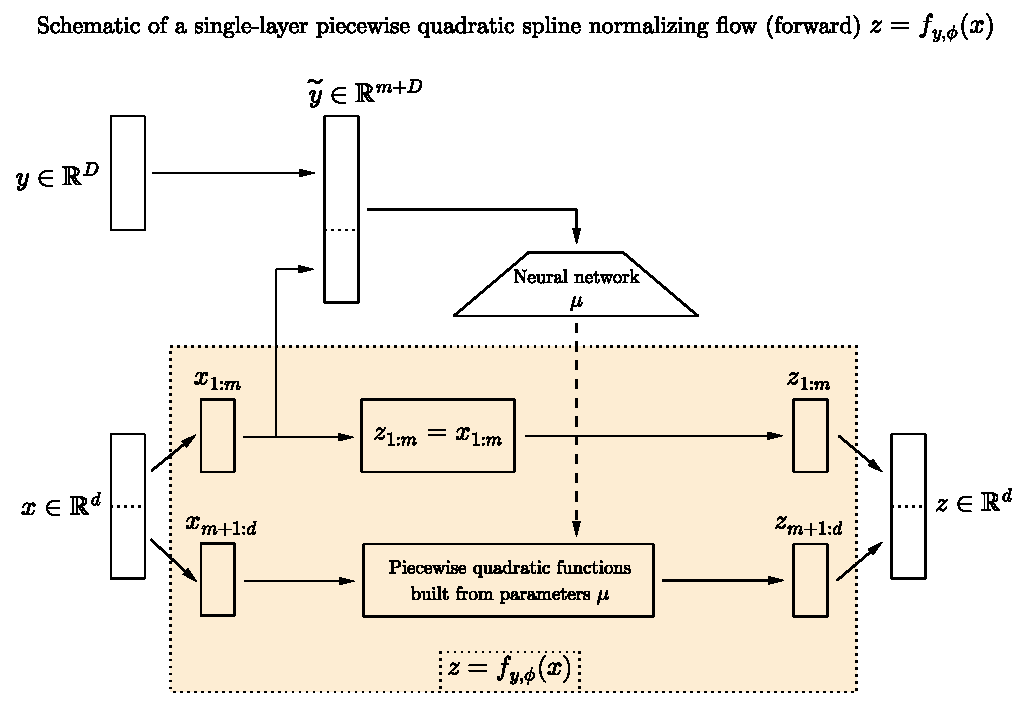
\includegraphics[width=0.8\textwidth]{figures/thesis/piecewisequadraticsplineflow_forward.pdf}
		\caption{Single-layer piecewise quadratic spline (coupling layer) normalizing flow (forward).}
		\label{fig:nflowquadratic_forward}
	\end{figure}
\end{frame}

\begin{frame}[allowframebreaks]{Appendix}
	\vspace{-0.5cm}
	\framesubtitle{Piecewise quadratic spline coupling layer flows}
	\begin{figure}[h]
		\centering
		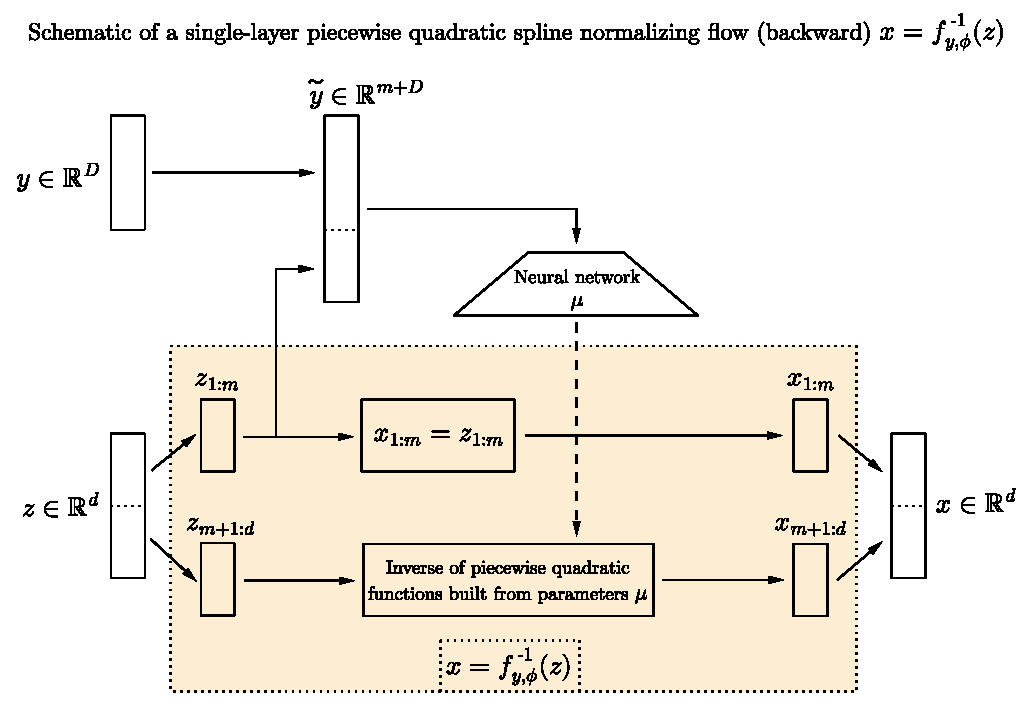
\includegraphics[width=0.8\textwidth]{figures/thesis/piecewisequadraticsplineflow_backward.pdf}
		\caption{Single-layer piecewise quadratic spline (coupling layer) normalizing flow (backward).}
		\label{fig:nflowquadratic_backward}
	\end{figure}
\end{frame}

\begin{frame}[allowframebreaks]{Appendix}
	\framesubtitle{What has been done yet using normalizing flows?}
	Normalizing flows were introduced in 2015 by \cite{Rezende.21.05.2015} as a new solution to approximate posterior probability densities $p(\vect{x}|\vect{y})$.
	
	A first attempt to apply normalizing flows as generative model for image modeling was made by \cite{Dinh.27.05.2016} in 2016. They demonstrated that normalizing flows can generate very similar images as those they were trained on.
	
	\cite{Durkan.10.06.2019} introduced the piecewise rational quadratic spline coupling layer flows and showed, that they are very flexible for approximating multimodal posterior densities.
\end{frame}


\begin{frame}[allowframebreaks]{Appendix}
	\framesubtitle{What has been done yet using normalizing flows?}
	Finally, \cite{DiazBaso.2022} applied normalizing flows to learn stellar atmospheric inversions. They successfully trained and evaluated normalizing flows using the scalar Milne-Eddington (no magn. field parameters) and a more complex non-LTE atmospheric model.
	
	The thesis at hand comes in here to explore normalizing flows applied to learn the full Milne-Eddington inversion task (with magn. field parameters).
\end{frame}

\begin{frame}[allowframebreaks]{Appendix}
	\framesubtitle{Change of variable formula}
	The change of variable formula is the centerpiece of the normalizing flow technique. 
	
	Suppose that $\vect{x}$, $\vect{z}$ $\in \mathbb{R}^d$ are multidimensional random variables with associated probability densities $p_{\vect{x}}(\vect{x})$ and $p_{\vect{z}}(\vect{z})$. Let furthermore $\vect{f}$ be a function transferring the variable $\vect{x}$ into $\vect{z}$ as $\vect{z} = \vect{f}(\vect{x})$.
	
	\cite[p.196]{Deisenroth.2020} give the change of variable theorem as \begin{align}\begin{aligned}
			p_{\vect{x}}(\vect{x}) = p_{\vect{z}}[\vect{f}(\vect{x})]\left|\det\left(\frac{\partial \vect{f}(\vect{x})}{\partial \vect{x}}\right)\right|.
	\end{aligned}\end{align}
\end{frame}

\begin{frame}[allowframebreaks]{Appendix}
	\framesubtitle{Principle/requirements of/for a normalizing flow}
	Suppose, that a function $\vect{f}: \mathbb{R}^d \rightarrow \mathbb{R}^d, \,\vect{x} \mapsto \vect{z} = \vect{f}(\vect{x})$ is a normalizing flow ($p_{\vect{z}}(\vect{z})$ being a standard normal distribution). The normalizing flow can be composed of several functions $\vect{f}_{(k)}$ such that $\vect{z} = \vect{f}(\vect{x}) = \vect{f}_{(n)} \circ \dots \circ \vect{f}_{(1)}(\vect{x})$.
	
	\cite{Kobyzev.2021} give three key requirements to the $\vect{f}_{(k)}$ such that they indeed compose a normalizing flow:
	\begin{enumerate}
		\item All $\vect{f}_{(k)}$ need to be invertible and differentiable.
		\item The transformations $\vect{f}_{(k)}$ need to be expressive enough to model complex data distributions.
		\item The transformations $\vect{f}_{(k)}$ are ideally computationally efficient, such that the computation of the Jacobian requires as little resources as possible.
	\end{enumerate}
\end{frame}

\begin{frame}[allowframebreaks]{Appendix}
	\framesubtitle{Moons experiment: Explanation}
	As an instructive example, an affine coupling layer normalizing flow was trained to map samples from a 2D ``moons'' target distribution to a 2D standard normal base distribution, as visualized in \cref{fig:target-to-base}.
	
	\begin{figure}
		\centering
		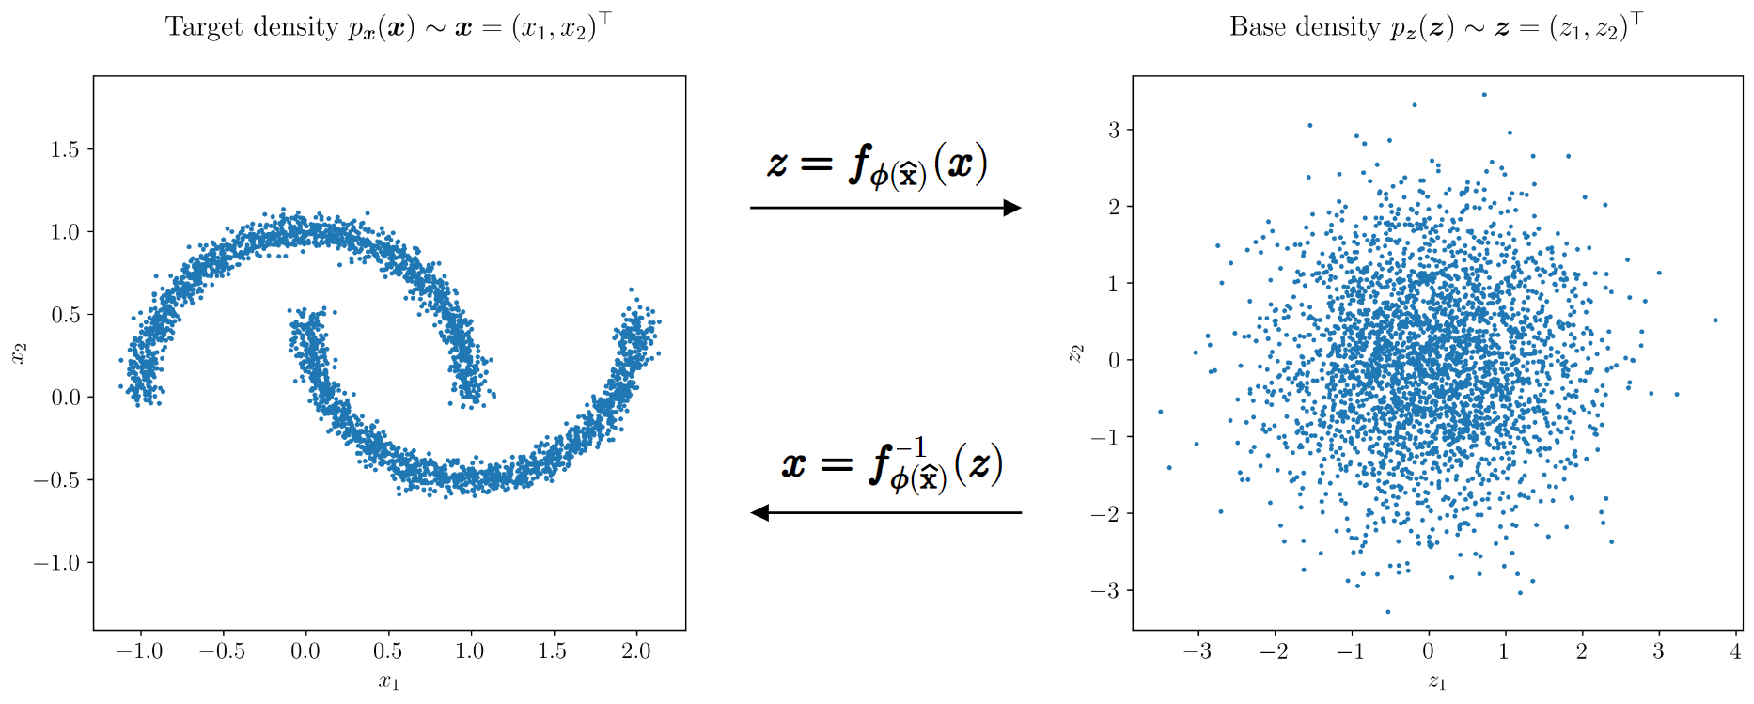
\includegraphics[width=0.87\textwidth]{figures/thesis/target-to-base.pdf}
		\caption{Visualization of a normalizing flow mapping the moons distribution to a standard normal distribution and vice versa in a plane.}
		\label{fig:target-to-base}
	\end{figure}
\end{frame}

\begin{frame}[allowframebreaks]{Appendix}
	\framesubtitle{Moons experiment: Explanation}
	The goal was to find a diffeomorphic (differentiable and invertible) function mapping a 2D standard normal distribution $\vect{z}$ to the distribution points $\vect{x}$ of the moons distribution as visualized in \cref{fig:moonsgoal}.
	\begin{figure}[h]
		\centering
		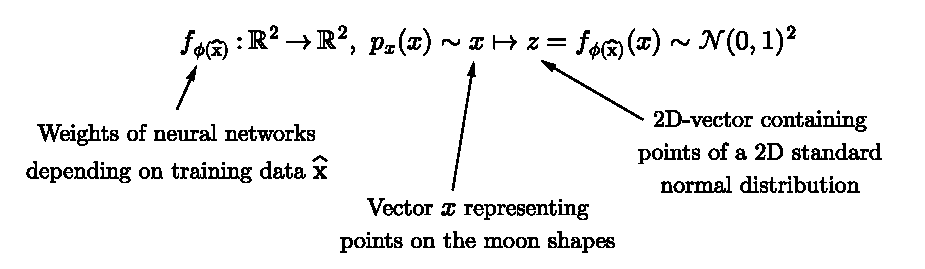
\includegraphics[width=\textwidth]{figures/presentation/moons.pdf}
		\caption{Goal for the normalizing flow applied to the moons experiment.}
		\label{fig:moonsgoal}
	\end{figure}
\end{frame}

\begin{frame}[allowframebreaks]{Appendix}
	\framesubtitle{Moons experiment: Results}
	\begin{figure}[h!]
		\centering
		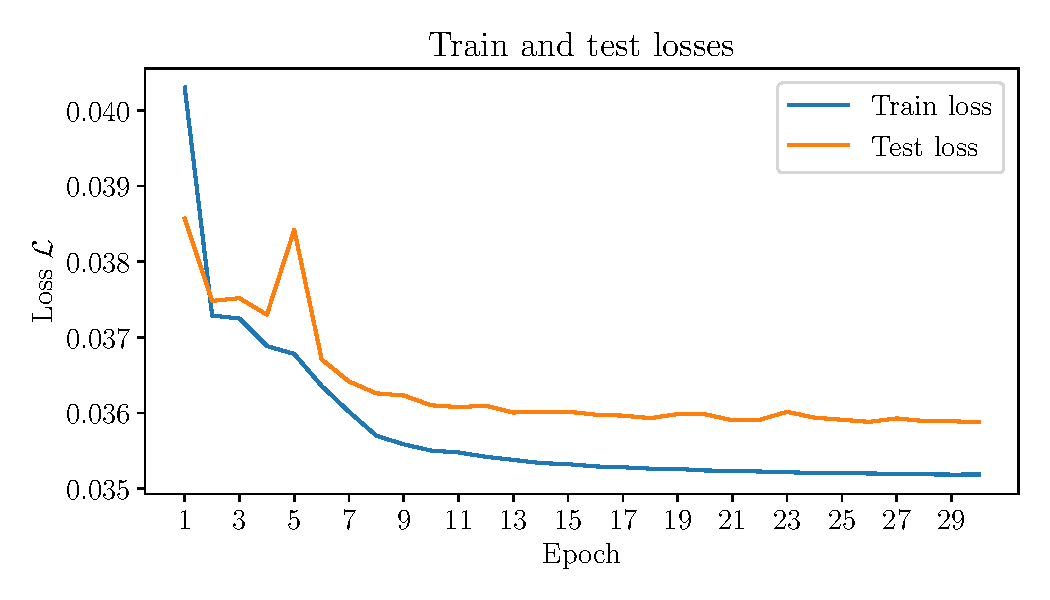
\includegraphics[width=8cm]{figures/thesis/nf-moons-example-loss}
		\caption{Learning curves for the model implementing a map from the moons distribution to a two-dimensional standard normal distribution.}
		\label{fig:nf-moons-example-loss}
	\end{figure}
	
	\begin{figure}[h!]
		\centering
		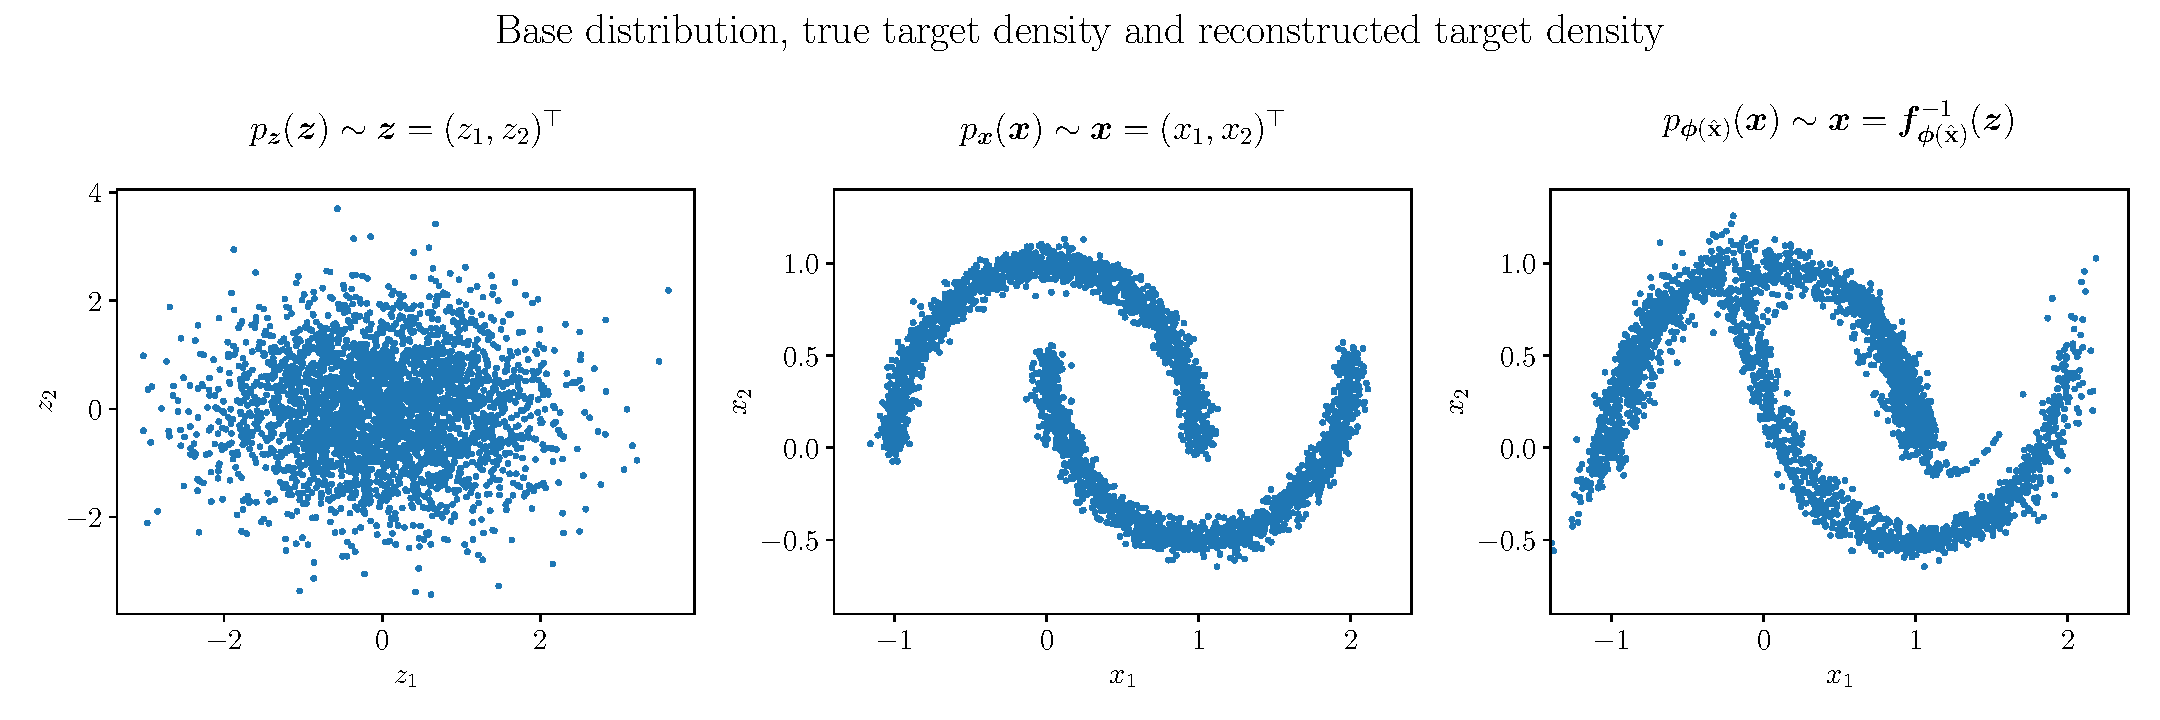
\includegraphics[width=\textwidth]{figures/thesis/nf-moons-example-plots.pdf}
		\caption{Results for a normalizing flow implementing a map from the moons distribution to a standard normal distribution in a plane (3000 samples).}
		\label{fig:nf-moons-example-plots}
	\end{figure}
\end{frame}

\begin{frame}[allowframebreaks]{Appendix}
	\framesubtitle{Moons experiment: Key features of results}
	There are three key points to take away from these results:
	\begin{enumerate}
		\item Model is possibly experiencing overfitting and potentially underrepresentativeness in training or testing data.
		\item The reconstructed target density features struggles to separate the two half-moons close to the origin.
		\item Generally speaking however, the normalizing flow technique seems to work as intended.
	\end{enumerate}
\end{frame}

\begin{frame}[allowframebreaks]{Appendix}
	\framesubtitle{Linear regression experiment: Explanation}
	\begin{columns}
		\begin{column}{0.49\textwidth}
			As an example, an affine coupling layer normalizing flow was trained on sets of parameters $\vect{x} = (a, b)^\top$ and associated lines (context) $\vect{y} = (y_1,\dots,y_{10})^\top$ with added noise.
			
			$\vect{x} \sim p_{\vect{x}}(\vect{x})$ and $\vect{y} \sim p_{\vect{y}}(\vect{y})$ are intertwined by $y_j = M_j(\vect{x}) = au_j + b$ for $j \in \{1,\dots,10\}$.
		\end{column}
		\begin{column}{0.49\textwidth}
			\begin{figure}[h]
				\centering
				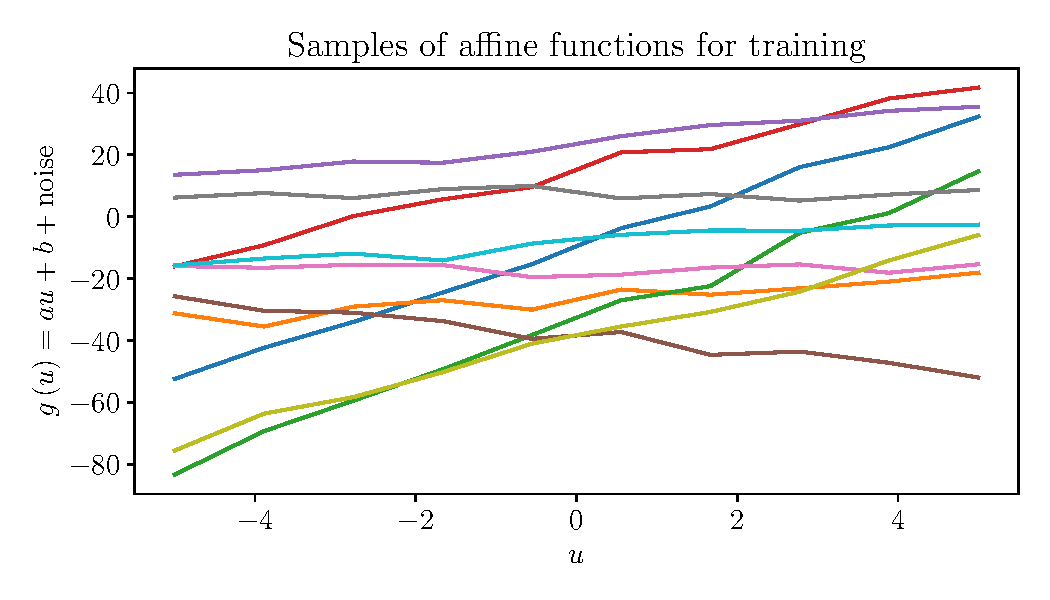
\includegraphics[width=\textwidth]{figures/thesis/nf-linear-regression-example-linesamples.pdf}
				\caption{Samples from the training dataset of context used in the linear regression example.}
				\label{fig:sample-lines}
			\end{figure}
		\end{column}
	\end{columns}
\end{frame}

\begin{frame}[allowframebreaks]{Appendix}
	\framesubtitle{Linear regression experiment: Explanation}
	The goal was to find a diffeomorphic (differentiable and invertible) function mapping a 2D standard normal distribution $\vect{z}$ to the distribution of linear regression parameters $\vect{x}$ as specified in \cref{fig:linearregressiongoal}.
	\begin{figure}[h]
		\centering
		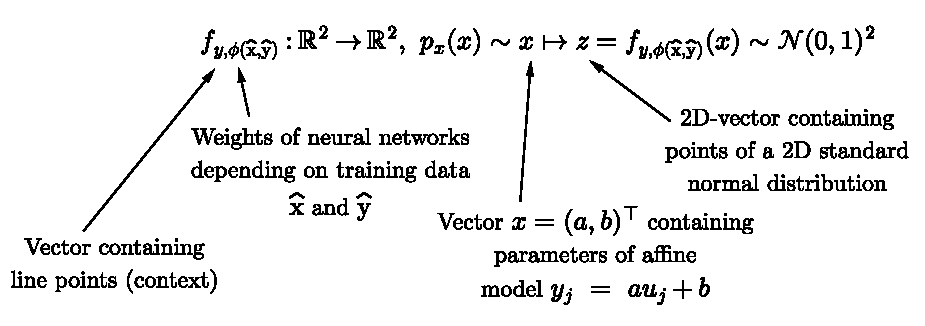
\includegraphics[width=\textwidth]{figures/presentation/linearregression.pdf}
		\caption{Goal for the normalizing flow applied to the linear regression experiment.}
		\label{fig:linearregressiongoal}
	\end{figure}
\end{frame}

\begin{frame}[allowframebreaks]{Appendix}
	\framesubtitle{Linear regression experiment: Results}
	\begin{figure}[h!]
		\centering
		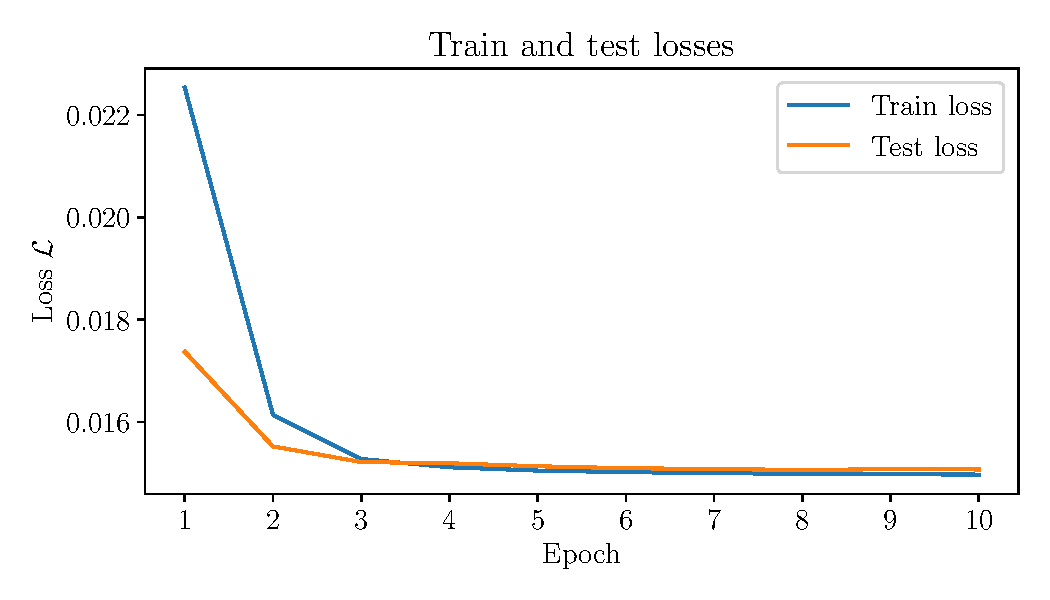
\includegraphics[width=8cm]{figures/thesis/nf-linear-regression-example-loss.pdf}
		\caption{Learning curves for the model implementing a map from parameter distributions of an affine function to a two-dimensional standard normal distribution, given the affine function values associated with the function parameters as context.}
		\label{fig:nf-linear-regression-example-loss}
	\end{figure}
	
	\begin{figure}[h!]
		\centering
		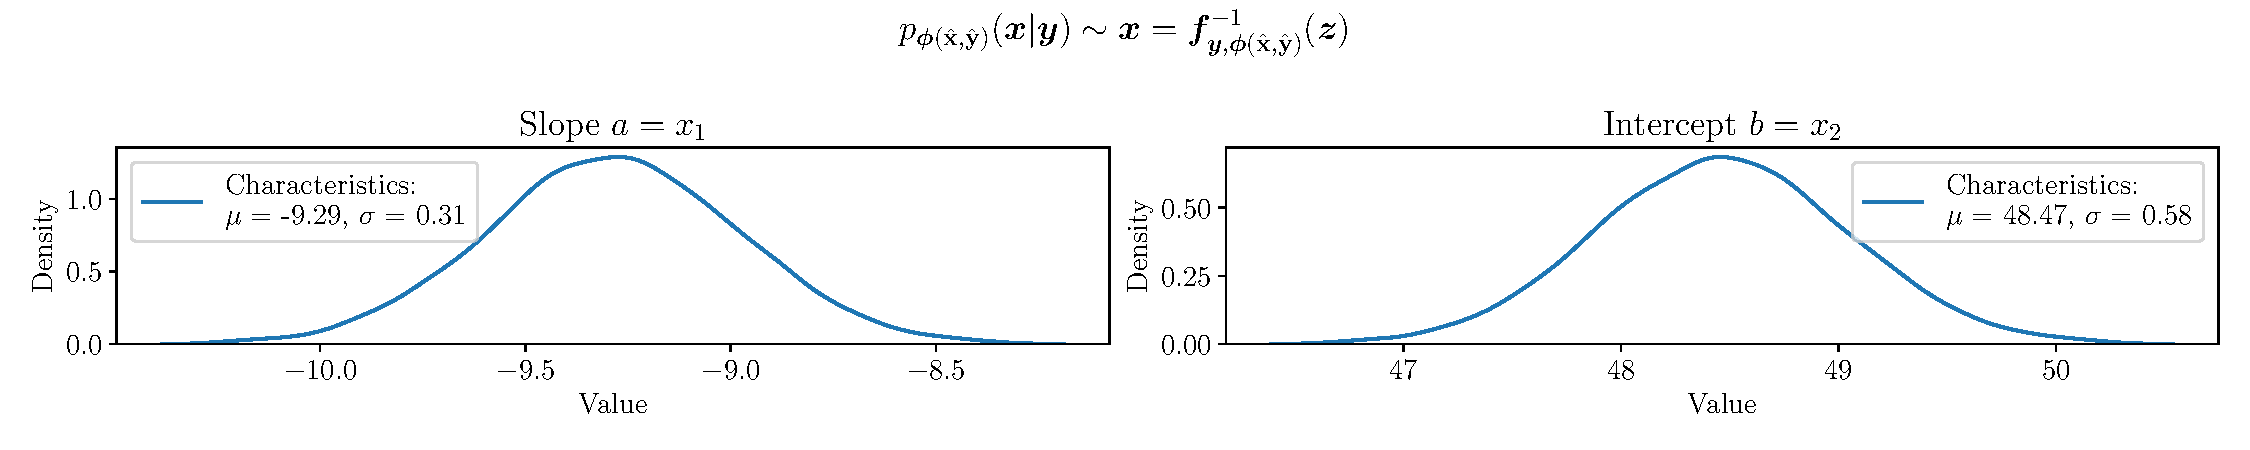
\includegraphics[width=0.8\textwidth]{figures/thesis/nf-linear-regression-example-calctargetdensities.pdf}
		\caption{Calculated densities for a test observation $\vect{y} = \vect{y}_{test}$ generated by parameters $\vect{x}_{test} = (-9.34, 47.64)^\top$ given to the normalizing flow.}
		\label{fig:nf-linear-regression-example-calctargetdensities}
	\end{figure}
	
	\begin{figure}[h!]
		\centering
		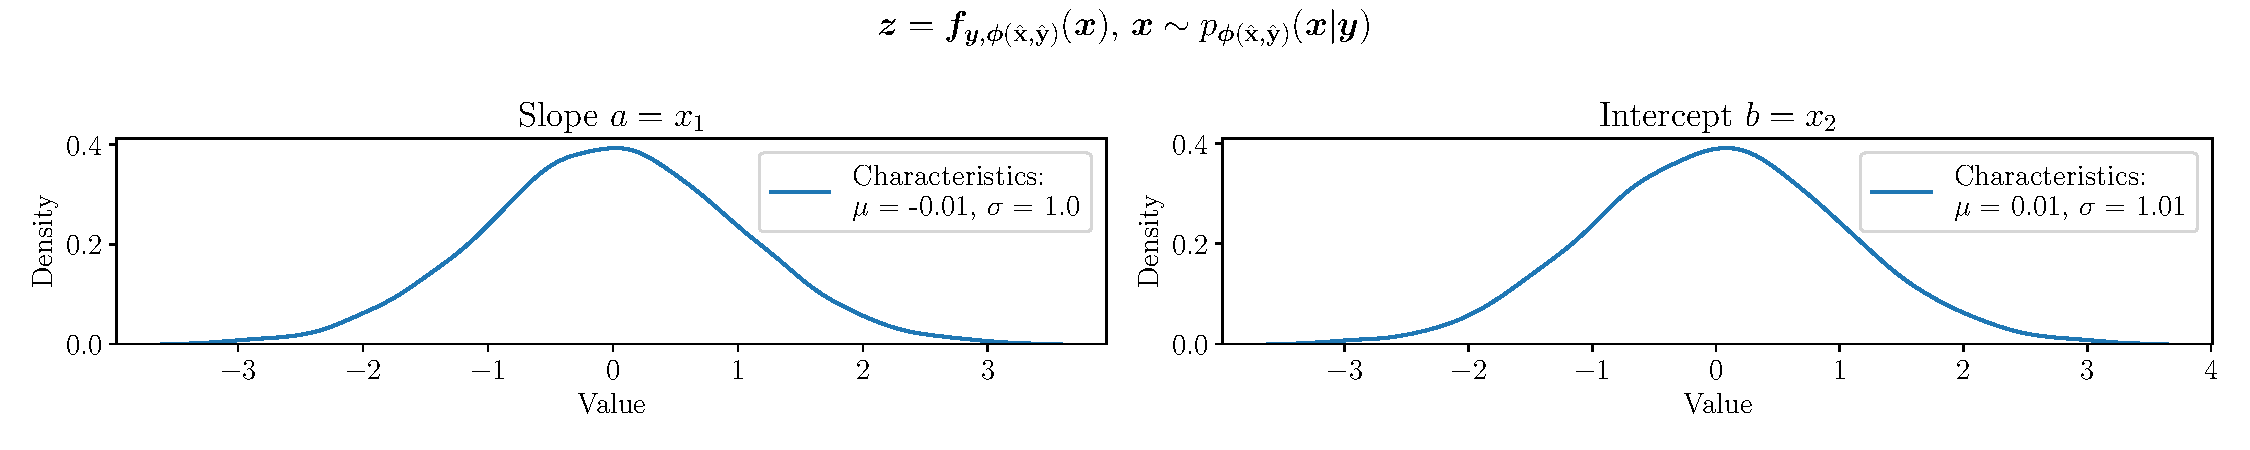
\includegraphics[width=0.8\textwidth]{figures/thesis/nf-linear-regression-example-calcbasedensities.pdf}
		\caption{Calculated latent densities for the parameter densities in the training dataset.}
		\label{fig:nf-linear-regression-example-calcbasedensities}
	\end{figure}
	
	\begin{figure}[h!]
		\centering
		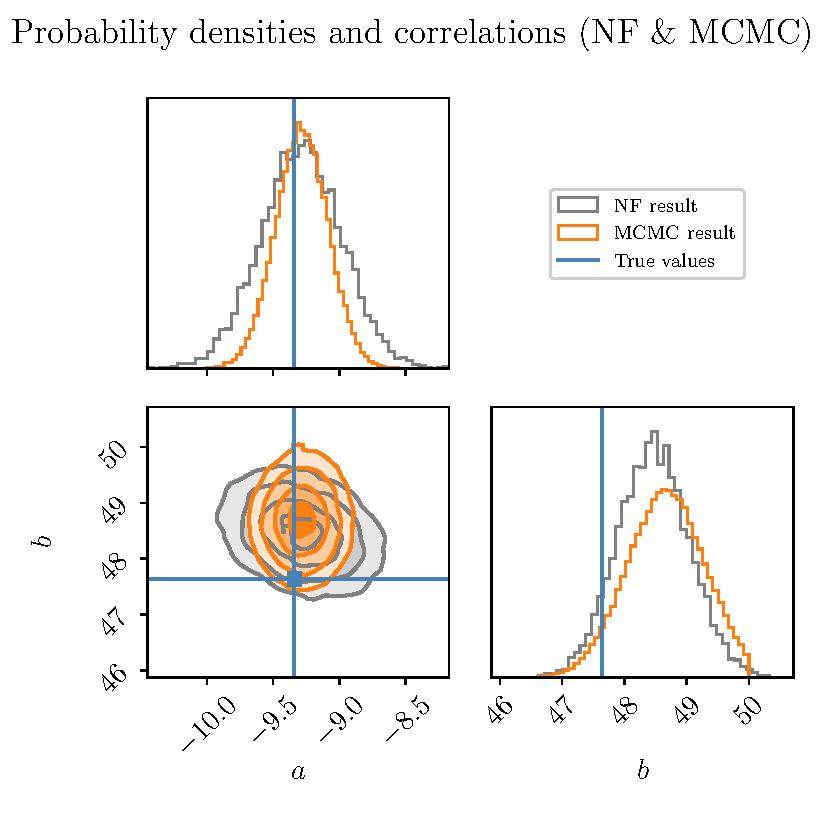
\includegraphics[width=0.49\textwidth]{figures/thesis/nf-linear-regression-example-corner-mcmc-nf.pdf}
		\caption{Comparison of normalizing flow (NF) and Markov Chain Monte Carlo simulation (MCMC) results for a test observation $\vect{y} = \vect{y}_{test}$ generated by test parameters $\vect{x} = \vect{x}_{test}$.}
		\label{fig:nf-linear-regression-example-corner-mcmc-nf}
	\end{figure}
	
	\begin{figure}[h!]
		\centering
		\begin{subfigure}[t]{0.49\textwidth}
			\centering
			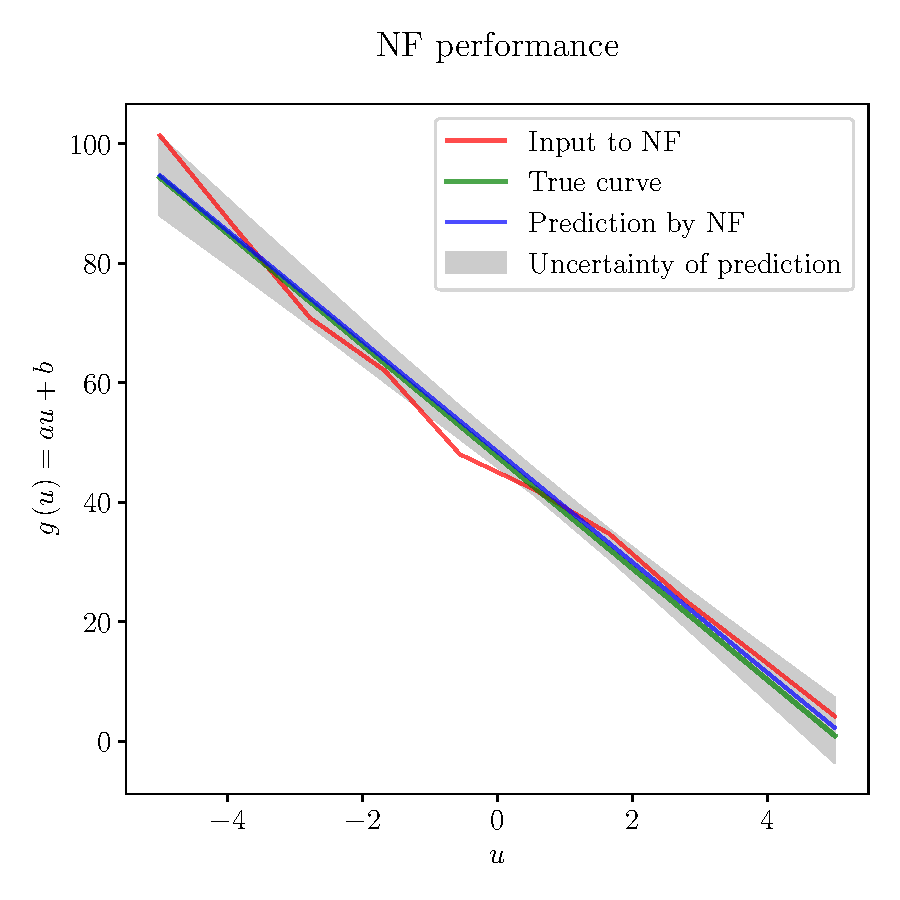
\includegraphics[width=\textwidth]{figures/thesis/nf-linear-regression-example-nfperformance.pdf}
		\end{subfigure}
		\hfill
		\begin{subfigure}[t]{0.49\textwidth}
			\centering
			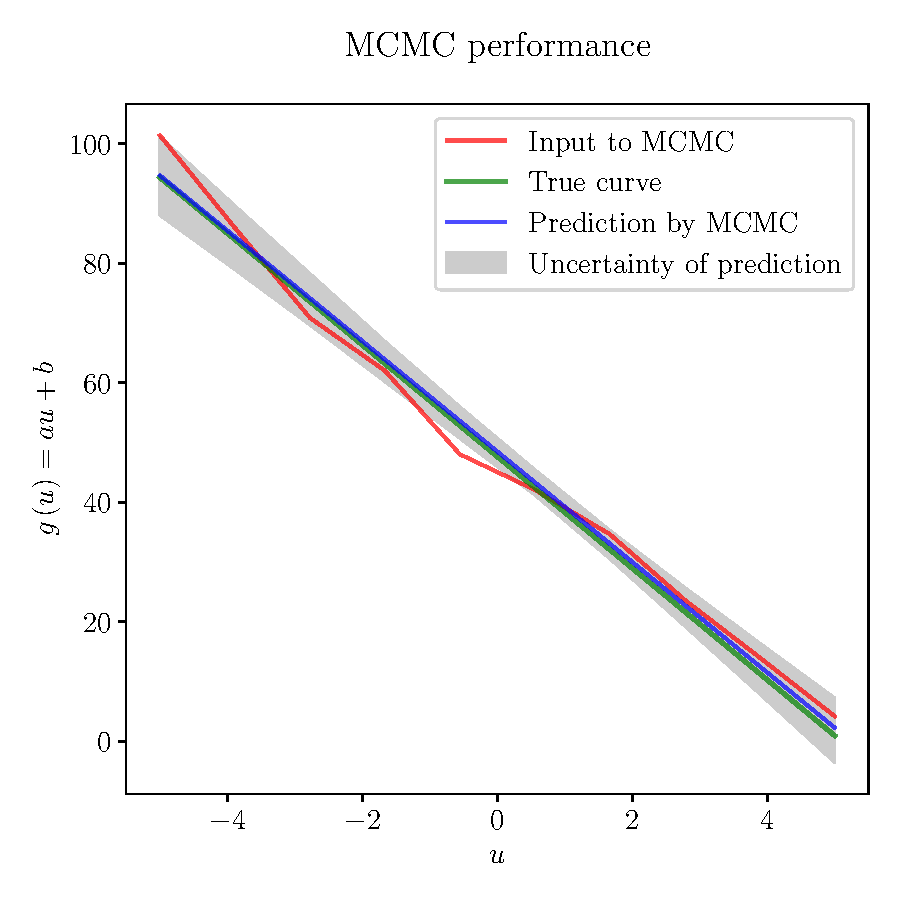
\includegraphics[width=\textwidth]{figures/thesis/nf-linear-regression-example-mcmcperformance.pdf}
		\end{subfigure}
		\caption{Left panel: Results obtained by the normalizing flow (NF) for $\vect{y} = \vect{y}_{test}$ and $\vect{x} = \vect{x}_{test}$. Right panel: Results obtained by the Markov Chain Monte Carlo simulation (MCMC) for the same test observation $\vect{y}_{test}$.}
		\label{fig:nf-linear-regression-example-performance}
	\end{figure}
\end{frame}

\begin{frame}[allowframebreaks]{Appendix}
	\framesubtitle{Linear regression experiment: Results}
	There are three key points to take away from these results:
	\begin{enumerate}
		\item The prediction by the normalizing flow almost everywhere partially to fully overlaps with the true curve.
		\item The prediction and uncertainty regions as obtained by the normalizing flow agree with those obtained by the Markov Chain Monte Carlo simulation.
		\item The uncertainty region and the prediction itself seems to fit well with the input data, on which the linear regression was carried out.
	\end{enumerate}
\end{frame}

\begin{frame}[allowframebreaks]{Appendix}
	\framesubtitle{Multiple map analysis using a different map for training: Experiment explanation} % Experiment 4
	This experiment basically was carried out as the previous experiment, but instead of using frame 0 of the penumbra formation dataset for training, a frame from a different active region of the sun was used (Stokes profiles $\hat{\matr{y}}$ and associated atmospheric parameters $\hat{\matr{x}}$ obtained by the Milne-Eddington algorithm).
	
	Once trained, the normalizing flow was applied to invert frames from the penumbra formation dataset.
	\begin{figure}[h!]
		\centering
		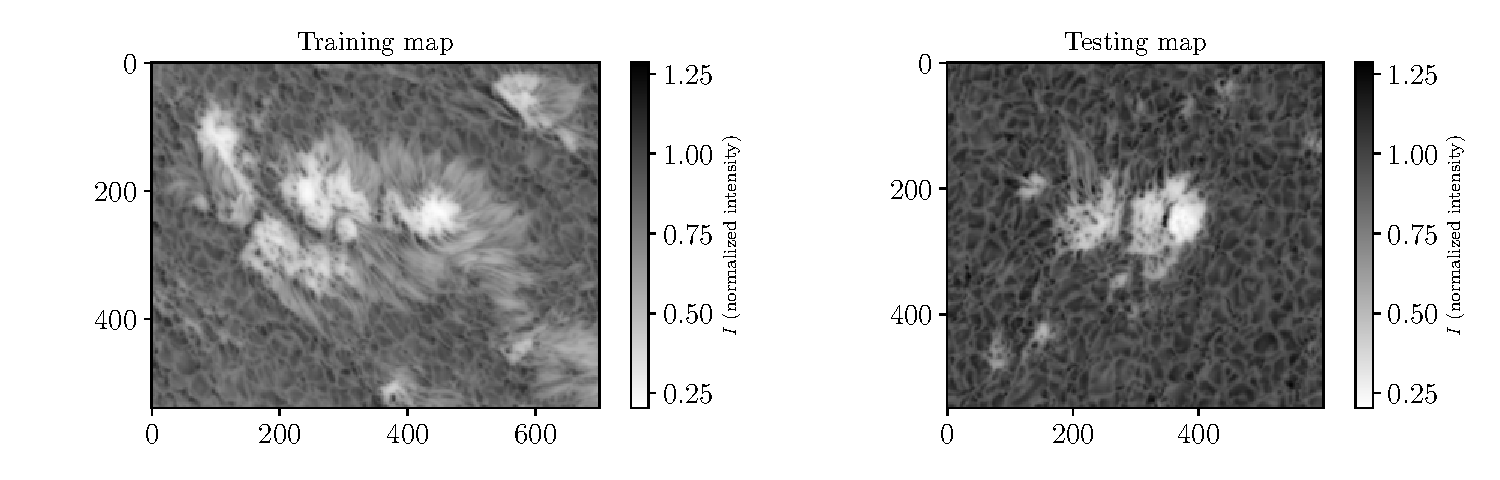
\includegraphics[width=\textwidth]{figures/thesis/nf-milne-eddington-example-4-trainingmap-testingmap-nflows-piecewisequadratic.pdf}
		\caption{Left panel: Frame used for training the normalizing flow. Right panel: Frame to be inverted by trained normalizing flow.}
		\label{fig:nf-milne-eddington-example-4-trainingmap-testingmap-nflows-piecewisequadratic}
	\end{figure}
\end{frame}

\begin{frame}[allowframebreaks]{Appendix}
	\framesubtitle{Multiple map analysis using a different map for training: Results} % Experiment 4
	\begin{figure}[h]
		\centering
		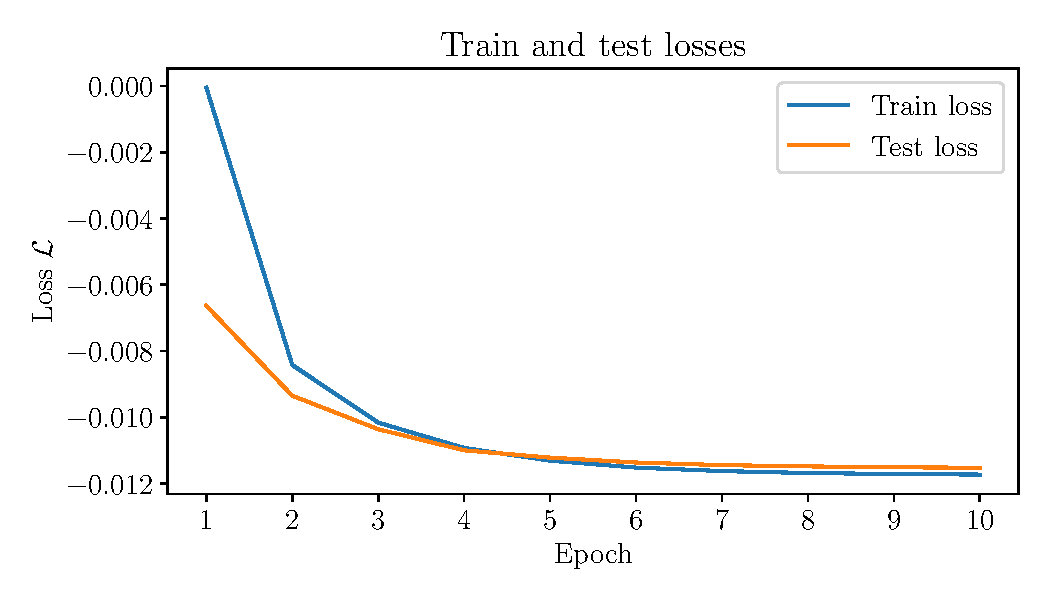
\includegraphics[width=8cm]{figures/thesis/nf-milne-eddington-example-4-loss-nflows-piecewisequadratic.pdf}
		\caption{Learning curve for experiment 4 of normalizing flows applied to learn Milne-Eddington inversions.}
		\label{fig:nf-milne-eddington-example-4-loss-nflows-piecewisequadratic}
	\end{figure}
\end{frame}

\begin{frame}[allowframebreaks]{Appendix}
	\framesubtitle{Multiple map analysis using a different map for training: Results} % Experiment 4
	\begin{figure}
		\begin{minipage}[c]{0.67\textwidth}
			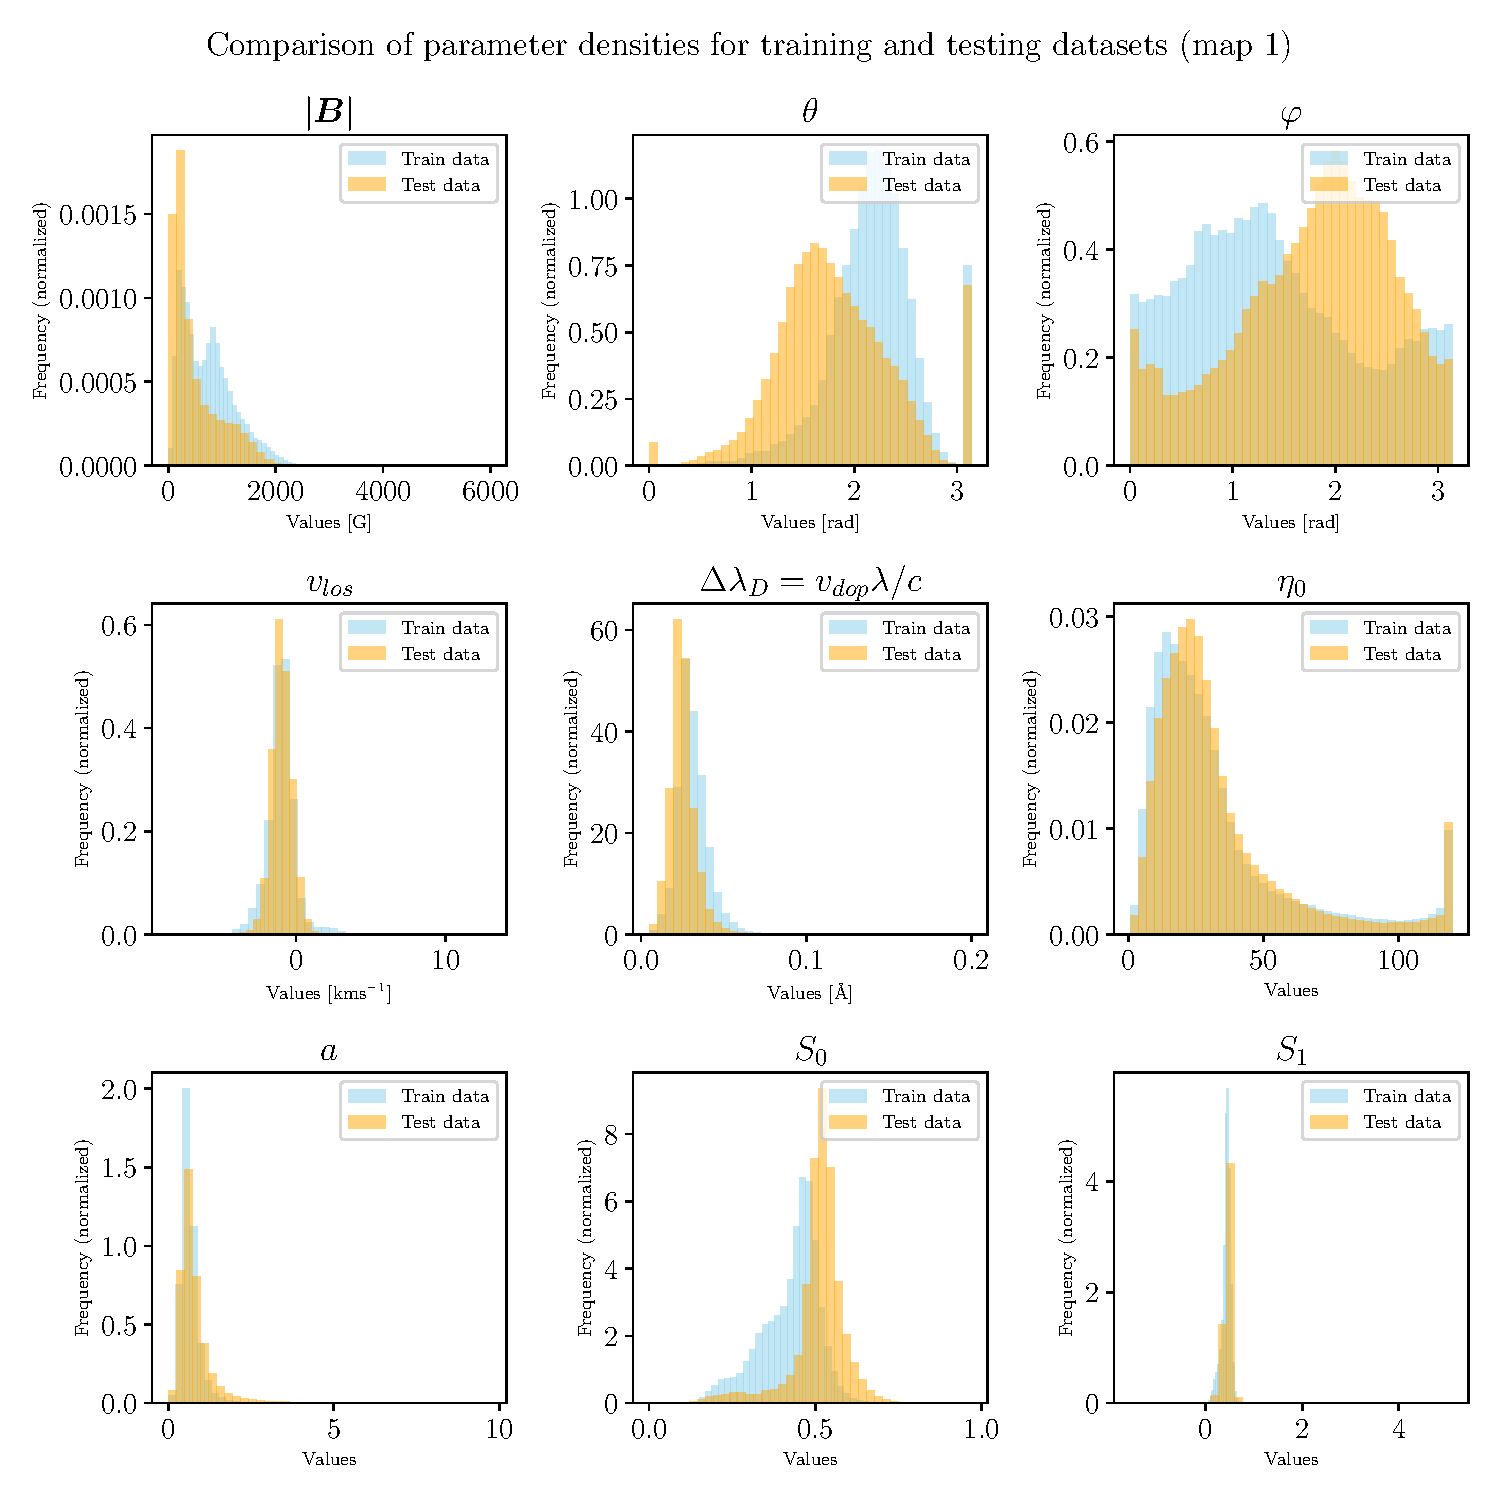
\includegraphics[width=\textwidth]{figures/thesis/nf-milne-eddington-example-4-nflows-piecewisequadratic-comp-paramdens-traintest-1.pdf}
		\end{minipage}\hfill
		\begin{minipage}[c]{0.3\textwidth}
			\caption{Visualization of variations in training and testing data. This plot shows data from the sunspot map as training data; and data of frame 0 (test map 1) from the penumbra formation dataset as testing data.
			} \label{fig:nf-milne-eddington-example-4-nflows-piecewisequadratic-comp-paramdens-traintest-1}
		\end{minipage}
	\end{figure}
\end{frame}

\begin{frame}[allowframebreaks]{Appendix}
	\vspace{-0.4cm}
	\framesubtitle{Multiple map analysis using a different map for training: Results} % Experiment 4
	\begin{figure}[h!]
		\centering
		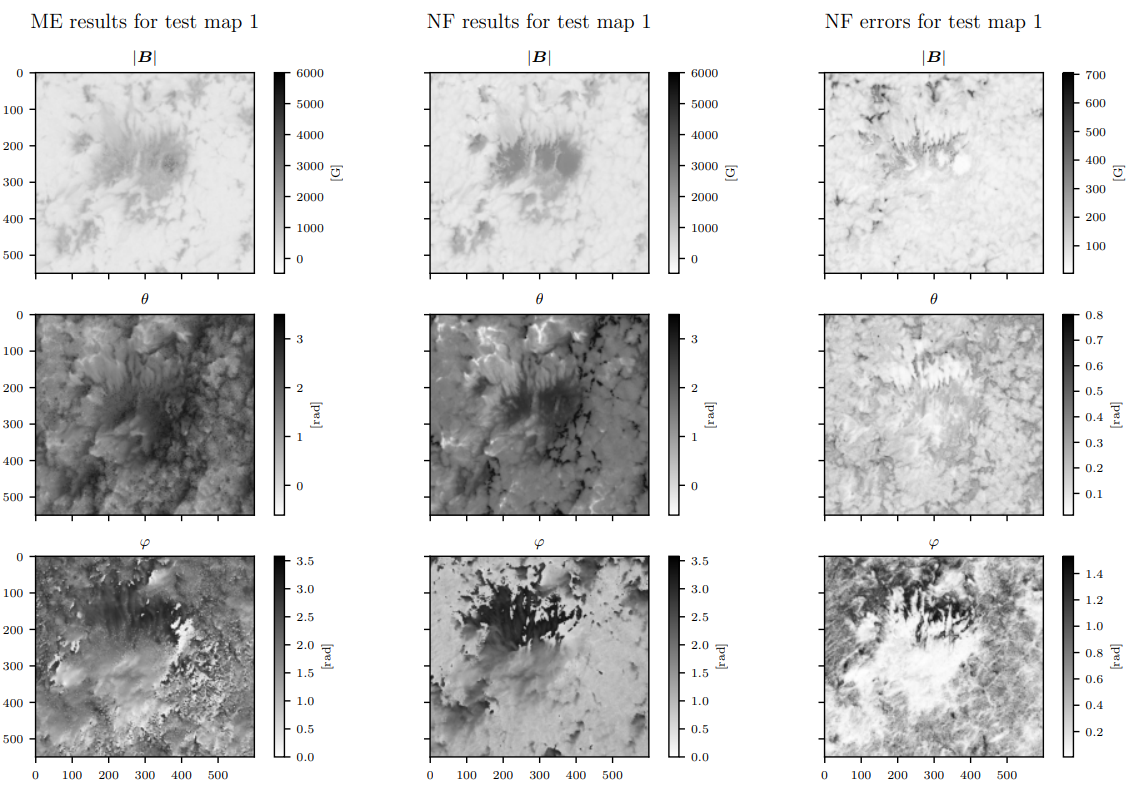
\includegraphics[width=8cm]{figures/presentation/exp4_fig1.png}
		\caption{Results for multiple map analysis using a different map for training experiment.}
		\label{fig:exp4_fig1}
	\end{figure}
\end{frame}

\begin{frame}[allowframebreaks]{Appendix}
	\vspace{-0.4cm}
	\framesubtitle{Multiple map analysis using a different map for training: Results} 
	There are three key points to take away from these results:
	\begin{enumerate}
		\item The training and testing losses show nearly ideal behaviour; after about 7 epochs, they seem to converge to a nearly constant value with little spacing.
		\item The ``smoothing property'' seems to be stronger in this case than in the previous case.
		\item Results for magnetic field parameters are of similar quality than in the previous case, except for the azimuth parameter $\varphi$.
	\end{enumerate}
\end{frame}

\begin{frame}[allowframebreaks]{Appendix}
	\framesubtitle{Tracking parameter evolution during penumbra formation: Experiment explanation} % Experiment 6
	For this experiment, the observational data $\hat{\matr{y}}$ and the associated parameter data $\hat{\matr{x}}$ of frame 0 was used to train a normalizing flow.
	
	Using this trained flow, all subsequent frames of the penumbra formation dataset were inverted.
	
	In the penumbra formation dataset, a penumbra can be observed to form in the area of the red rectangle in \cref{fig:nf-milne-eddington-example-7-considered-map-section-nflows-piecewisequadratic}.
	
	\begin{figure}[h!]
		\centering
		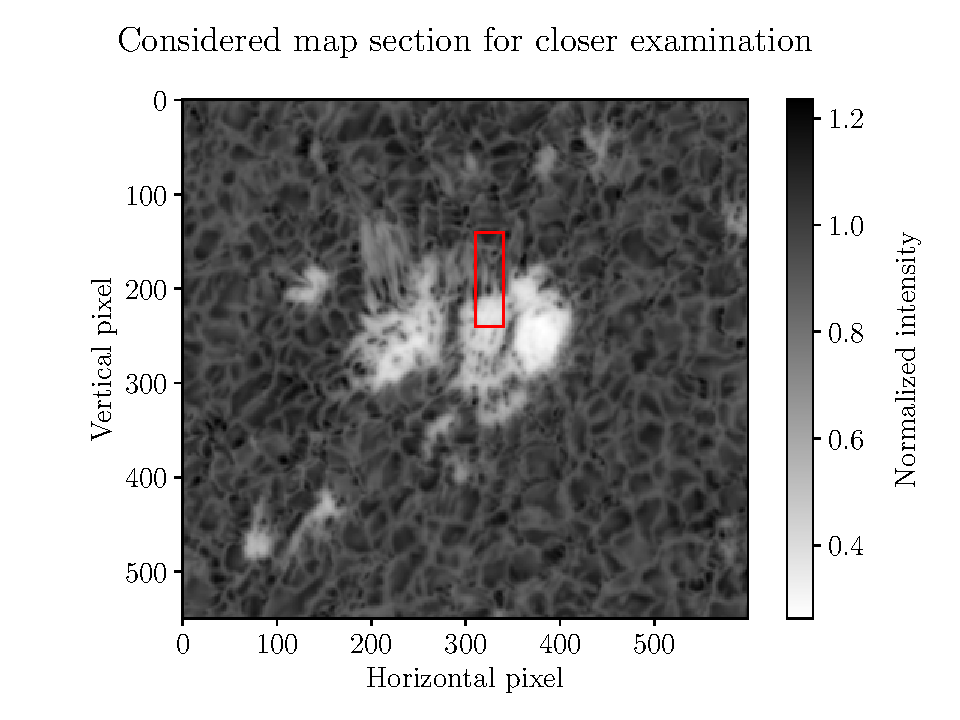
\includegraphics[width=8cm]{figures/thesis/nf-milne-eddington-example-7-considered-map-section-nflows-piecewisequadratic.pdf}
		\caption{Area of particular interest for atmospheric parameter evolution during penumbra formation.}
		\label{fig:nf-milne-eddington-example-7-considered-map-section-nflows-piecewisequadratic}
	\end{figure}
\end{frame}

\begin{frame}[allowframebreaks]{Appendix}
	\framesubtitle{Tracking parameter evolution during penumbra formation: Results} % Experiment 6, learning curve
	\begin{figure}[h!]
		\centering
		\includegraphics[width=8cm]{figures/thesis/nf-milne-eddington-example-7-loss-nflows-piecewisequadratic.pdf}
		\caption{Train and test losses of normalizing flow training process for parameter evolution experiment.}
		\label{fig:nf-milne-eddington-example-7-loss-nflows-piecewisequadratic}
	\end{figure}
\end{frame}

\begin{frame}[allowframebreaks]{Appendix}
	\framesubtitle{Tracking parameter evolution during penumbra formation: Results} % Experiment 6, red rectangle results
	\vspace{-0.5cm}
	\begin{figure}[h!]
		\centering
		\includegraphics[width=8.2cm]{figures/presentation/exp6_fig1.png}
		\caption{Results for parameter evolution experiment.}
		\label{fig:exp6_fig1}
	\end{figure}
\end{frame}

\begin{frame}[allowframebreaks]{Appendix}
	\framesubtitle{Tracking parameter evolution during penumbra formation: Results} % Experiment 6, penumbra formation sketch
	\begin{figure}[h!] % Leave this picture here
		\centering
		\includegraphics[width=\textwidth]{figures/thesis/penumbraformation.pdf}
		\caption{Schematic of what is expected to happen to the magnetic field lines during the penumbra formation process. Note, that the magnetic field lines as drawn here could also be oriented exactly opposite, i.e. facing towards the Sun's interior.}
		\label{fig:penumbraformation}
	\end{figure}
\end{frame}

\begin{frame}[allowframebreaks]{Appendix}
	\framesubtitle{Tracking parameter evolution during penumbra formation: Results} % Experiment 6
	There are two key points to take away from these results:
	\begin{enumerate}
		\item Train and test loss curves show a desirable behaviour indicating, that the model has indeed learned the characteristic properties of Milne-Eddington inversions.
		\item The evolution of magnetic field parameters as obtained by a normalizing flow inversion seems to match expectations.
	\end{enumerate}
\end{frame}
% Add table with hyperparameters to every experiment.

\end{document}

